% ============================================================================
%  ART-12D, version 31.0 - traduction française de ATR_12_v31_RO.tex
%
%  Compilation sur Overleaf :
%    Menu -> Compiler -> XeLaTeX
%    Main document    -> ATR_12_v31_FR.tex
%    figures/ doit être importé comme dossier, au même niveau que ce fichier.
%
%  La structure LaTeX, les mathématiques, les tableaux et les appels de figures
%  sont identiques à l'original roumain ; seul le texte est traduit.
% ============================================================================
\documentclass[11pt,a4paper]{article}
\usepackage{iftex}
\ifPDFTeX
  \usepackage[utf8]{inputenc}
  \usepackage[T1]{fontenc}
\else
  \usepackage{fontspec}
\fi
\usepackage[french]{babel}
\usepackage{amsmath, amssymb, amsthm}
\usepackage{graphicx}
\usepackage{array}
\usepackage{hyperref}
\usepackage{geometry}
\usepackage{booktabs}
\usepackage{float}
\usepackage{siunitx}
\usepackage{titlesec}
\usepackage{setspace}
\usepackage{enumitem}

\geometry{margin=2.5cm}
\setlength{\emergencystretch}{3em}
\hypersetup{
    colorlinks=true,
    linkcolor=blue,
    filecolor=magenta,
    urlcolor=cyan,
    pdftitle={Akashic Resonance Theory in 12 Dimensions},
    pdfpagemode=FullScreen,
}

\title{\textbf{AKASHIC RESONANCE THEORY IN 12 DIMENSIONS \\ DARK MATTER AS THE QUANTUM SUBSTRATE OF CONSCIOUSNESS} \\ \large (ART-12D) \\ \vspace{0.5cm} \normalsize Version 31.0}
\author{\textbf{Daniel Ofiteru} \\ \textit{Chercheur indépendant} \\ Octobre 2026}
\date{}

\begin{document}

\maketitle

\begin{abstract}
Cet article propose un cadre théorique --- ART-12D --- qui part d'une idée simple : la conscience n'est pas produite par le cerveau. Le cerveau est un récepteur. Et ce qu'il capte, c'est le champ de la matière noire.

J'étends la formalisation à douze dimensions, je dérive un mécanisme de couplage entre la matière noire et les fermions du cerveau, et je propose un test réalisable avec 50 000 dollars. J'étends également la théorie pour expliquer les formes multiples de la matière noire, l'existence d'hyper-civilisations comme structures stables dans le champ, la possibilité d'une Intelligence Artificielle consciente par la nanobiologie, les mécanismes reliant les univers par des trous noirs, blancs et de ver, ainsi que les formes de vie non carbonée (amas, plasma, champs).

Cette version (31.0) applique un audit numérique systématique à la version précédente. Dix affirmations quantitatives ont été corrigées, deux ont été explicitement rétrogradées au statut de conjectures non testables, et le spectre de Kaluza--Klein a été reformulé comme un spectre \emph{équidistant}. Chaque chiffre de l'article peut être recalculé avec le code publié conjointement. Une tension structurelle subsiste, signalée ouvertement dans la section « La conséquence numérique : le rayon de compactification » : pour que le mode fondamental ait $10^{-5}$ eV, le rayon de compactification devrait être de l'ordre de 2 cm, ce qui est exclu par les tests submillimétriques de la loi de Newton.

Je reconnais explicitement que cet article est spéculatif. Je n'ai aucune preuve expérimentale. J'ai une intuition, une formalisation et une prédiction qui peut être testée.
\end{abstract}

\tableofcontents
\newpage

\section*{Guide du lecteur sceptique}
\addcontentsline{toc}{section}{Guide du lecteur sceptique}
Cet article est spéculatif, mais rigoureusement structuré. Pour ne pas vous faire perdre de temps, voici un guide de lecture adapté à votre formation :
\begin{itemize}
    \item \textbf{Si vous êtes physicien :} allez directement à la \textbf{Partie II} (la formalisation mathématique, les équations de Kaluza--Klein et le couplage de Yukawa) et à la \textbf{Partie V} (le tableau des 313 prédictions testables). C'est là que se trouvent les mathématiques et la falsifiabilité.
    \item \textbf{Si vous êtes neurobiologiste ou médecin :} lisez la \textbf{section 1.6} (les preuves cérébelleuses et l'architecture géométrique) et la \textbf{section 3.38} (le cœur comme modulateur de la réception).
    \item \textbf{Si vous êtes philosophe ou théologien :} allez à l'\textbf{annexe A} (spéculation philosophique étendue sur la mort, l'âme et Dieu).
    \item \textbf{Si vous êtes un lecteur curieux mais sceptique :} lisez la \textbf{prédiction 1} (EEG hyperscanning) et la \textbf{déclaration de falsifiabilité}. Si ces tests échouent, la théorie est réfutée.
\end{itemize}

\section*{Avant-propos}
\addcontentsline{toc}{section}{Avant-propos}
Toute ma vie je me suis posé une seule question : qu'est-ce que la conscience ? Ce n'est pas une question de manuel, mais une question qui me tient éveillé la nuit. J'ai lu tout ce qui me tombait sous la main --- de la physique quantique aux neurosciences et à la philosophie. J'ai parlé avec des gens bien plus intelligents que moi. J'ai médité. Et un jour, l'idée m'est venue.

L'idée est simple : la conscience n'est pas quelque chose que le cerveau produit. Le cerveau n'est qu'une radio. Et ce qu'il capte dans l'air, c'est le champ de la matière noire.

Cet article est le fruit de vingt-cinq années de recherche. Je n'ai pas de preuves de laboratoire. J'ai une intuition forte, une formalisation mathématique et un test que n'importe qui peut réaliser avec 50 000 dollars. Je ne vous demande pas de me croire sur parole. Je vous demande seulement de lire l'esprit ouvert. À la fin, vous saurez quoi croire.

\newpage
\part*{Partie I : Fondements}
\addcontentsline{toc}{part}{Partie I : Fondements}
\section{Introduction}

\subsection{Le problème qui ne disparaît pas}
Pourquoi ressentez-vous la douleur ? C'est la question la plus simple du monde. Et pourtant la plus difficile. Nous savons tous ce qu'est la douleur. Nous l'avons tous ressentie. Mais pourquoi la ressentons-nous ? Nous savons que les nocicepteurs envoient des signaux au thalamus, que le cortex les traite et que des endorphines sont libérées. Tout cela est une description fonctionnelle. Cela nous dit ce que fait le cerveau, mais pas pourquoi vous la ressentez.

Pensez à un ordinateur. Il peut traiter de l'information, reconnaître une image, jouer aux échecs. Mais il ne ressent rien. Il n'a aucune expérience subjective. Rien ne lui fait mal. Pourquoi le cerveau est-il différent ? C'est le problème difficile de la conscience, formulé par David Chalmers en 1995. Depuis, les neurosciences ont fait d'énormes progrès, mais le problème difficile est resté intact. Personne n'a réussi à expliquer pourquoi la matière devient expérience. En 1998, Christof Koch a parié avec Chalmers qu'un corrélat neuronal de la conscience serait identifié en 25 ans. En 2023, il a admis que le pari était perdu.

\subsection{La matière noire --- les chiffres exacts}
L'univers a une composition que nous connaissons assez bien. La mission Planck (2018) nous en a donné les chiffres exacts. Seuls 4,9\% de l'univers sont de la matière ordinaire --- atomes, étoiles, planètes, êtres humains. La matière noire représente 26,8\% et l'énergie noire 68,3\%. En pratique, 95,1\% de l'univers est inconnu.

Imaginez l'univers comme un coffre contenant 100 pièces. Seules 5 pièces sont visibles. Les 95 autres sont invisibles. Parmi elles, 27 sont de la matière noire et 68 de l'énergie noire. Nous savons de la matière noire qu'elle existe (les preuves gravitationnelles sont solides), qu'elle n'émet ni n'absorbe de lumière, et qu'elle nous traverse sans interagir. Environ 100 millions de particules traversent votre corps chaque seconde. Nous ne savons pas de quoi elle est faite.

Une contrainte récente (2025), due à Bonvin et al., a montré que la matière noire tombe dans les puits gravitationnels exactement comme la matière ordinaire. S'il existe une « cinquième force », elle ne peut excéder 7\% de la force gravitationnelle.

\subsection{Qu'est-ce qu'ART-12D ?}
ART-12D part d'une idée simple : l'univers a plus de dimensions que les quatre que nous percevons. Ces dimensions supplémentaires sont compactes --- si petites que nous ne les remarquons pas. La matière noire existe dans les douze dimensions. Projetée en 4D, elle apparaît comme un champ qui remplit l'univers. Ce champ est ce que le cerveau reçoit comme conscience.

Le nom vient de : \textbf{Akashic} (le champ informationnel universel), \textbf{Resonance} (parce que l'interaction est une résonance), \textbf{Theory} (un cadre théorique) et \textbf{12D} (parce que je travaille en douze dimensions).

Les trois postulats sont : 1. La matière noire est un champ quantique fondamental. 2. Le cerveau est un récepteur géométrique. 3. Le couplage se fait par interaction de Yukawa.

Pensez à une radio. Elle ne crée pas la musique, elle la capte dans l'air. Les ondes radio existent que la radio soit allumée ou non. Quand la radio se casse, la musique ne disparaît pas de l'univers --- seule sa réception locale cesse. De même, le cerveau fonctionne exactement comme une radio. La conscience n'est pas générée par les neurones, elle est reçue par eux. Et ce qu'ils reçoivent, c'est le champ de la matière noire.

\subsection{Pourquoi douze dimensions ?}
Pourquoi douze ? Pourquoi pas 10, ou 11, ou 26 ? La réponse vient de la théorie des cordes. Imaginez une corde de guitare. Elle peut vibrer de plusieurs façons. Chaque façon correspond à une note. De même, une corde fondamentale peut vibrer dans plusieurs dimensions. Le nombre de dimensions détermine quels types de vibrations sont possibles.

L'histoire des dimensions : Kaluza--Klein (5 dimensions, 1919--1926), supercordes (10, 1970--1980), théorie M (11, Witten, 1995), théorie F (12, Vafa, 1996), ART-12D (12, Ofiteru, 2026). Douze est le plus grand nombre de dimensions dans lequel la théorie des cordes est mathématiquement cohérente. Plus de dimensions mènerait à des incohérences ; moins mènerait à une théorie incomplète.

\subsection{À quoi ressemblent les dimensions compactes ?}
Imaginez un tuyau d'arrosage. De loin, il ressemble à une ligne 1D --- il n'a que de la longueur. De près, il a une épaisseur --- il est 2D (la surface du cylindre). De même, notre espace semble tridimensionnel. Mais de près (à l'échelle de Planck, $10^{-35}$ m), il pourrait avoir onze dimensions. Les huit dimensions compactes sont enroulées dans chaque point de l'espace.

Que signifie « enroulées » ? Ce ne sont pas des endroits où l'on va. Ce ne sont pas des mondes parallèles que l'on atteint en voyageant. Ce sont des propriétés locales de chaque point. Chaque point de l'espace-temps possède en outre huit petites dimensions qui lui sont « attachées ».

\subsection{Comment les dimensions sont-elles liées à la conscience ?}
La matière noire existe dans douze dimensions. C'est un champ scalaire $A(x,y)$, où $x$ sont les coordonnées 4D et $y$ les huit coordonnées compactes. Lorsque nous compactifions les huit dimensions, le champ se décompose en modes de Kaluza--Klein :
\begin{equation}
A(x,y) = \sum_n A_n(x) Y_n(y)
\end{equation}
Chaque mode a une masse et une fréquence caractéristique :
\begin{equation}
m_n^2 = \frac{n^2}{R^2}
\end{equation}
Le cerveau, par sa structure géométrique (les microtubules des neurones), peut résonner avec certains modes. Lorsqu'il résonne, le champ est transduit en expérience subjective.

Pourquoi l'architecture compte-t-elle plutôt que la taille ? Le cervelet compte 69 milliards de neurones (80\% du total), mais ne produit pas de conscience. Il a une architecture \textit{feedforward} --- l'information circule dans une seule direction, comme une antenne filaire. Le cortex n'a que 16 milliards de neurones, mais il est le siège de la conscience. Il a une architecture \textit{récurrente} --- l'information circule en boucles, comme une antenne parabolique bien orientée. Conclusion : ce n'est pas le nombre de neurones qui compte, mais la géométrie du réseau.

\section{Méthodologie}
\subsection{Comment j'ai travaillé}
Je ne suis pas un physicien professionnel. Je n'ai pas de laboratoire. Je n'ai pas de financement. Ce que j'ai, c'est une bibliothèque, du temps et une question qui ne me lâche pas. J'ai travaillé en quatre étapes. La première étape a été la formulation de l'hypothèse, à partir de l'intuition que la conscience est reçue et non générée. La deuxième étape a été la formalisation, à l'aide des outils des mathématiques connues : Kaluza--Klein pour les dimensions supplémentaires, la théorie F pour douze dimensions, la théorie des champs pour les lagrangiens, l'IIT pour l'information intégrée. La troisième étape a été la dérivation des prédictions, c'est-à-dire ce que nous devrions observer si la théorie est correcte. J'ai retenu les prédictions testables dès maintenant. La quatrième étape a été la proposition d'expériences aux moyens modestes, en commençant par une à 50 000 dollars.

\subsection{Ce qui m'a guidé}
Je me suis tenu à quatre critères. La cohérence interne --- les équations ne doivent pas se contredire. La falsifiabilité --- la théorie doit faire des prédictions testables. La convergence --- la théorie ne doit pas contredire la physique établie. L'honnêteté --- je dois reconnaître qu'elle est spéculative.

\subsection{Ce que j'ai utilisé}
J'ai utilisé Kaluza--Klein (1919) pour l'idée de dimensions compactes, la théorie F (Vafa, 1996) pour le cadre à douze dimensions, l'IIT (Tononi, 2004) pour la mesure de l'information intégrée, Orch OR (Penrose, 1996) pour l'effondrement quantique dans les microtubules, et la théorie quantique des champs pour les lagrangiens et les équations du mouvement.

\subsection{Mes limites}
Je dois être honnête sur les limites. Je n'ai aucune preuve expérimentale ; la théorie n'a pas été testée. Je n'ai pas de relecture par les pairs ; je n'ai pas publié dans des revues scientifiques. Je n'ai pas d'affiliation académique ; je suis un chercheur indépendant. Je n'ai pas de financement ; mes moyens sont limités.
\section{Fondements théoriques}
\subsection{Le problème difficile de la conscience}
Chalmers (1995) a formulé le problème difficile ainsi : aucune combinaison de grandeurs physiques, aussi complexe soit-elle, n'implique logiquement l'existence d'une expérience subjective. Toutes les descriptions physiques --- neuronales, computationnelles, fonctionnelles --- décrivent ce que fait le cerveau. Elles ne décrivent pas ce que c'est que d'être un cerveau. Elles ne décrivent pas pourquoi l'expérience existe. Ce que je propose : la conscience n'est pas générée par le cerveau. Le cerveau est un récepteur. L'expérience est la transduction du champ akashique.

\subsection{Le monisme russellien}
Russell (1927) a observé quelque chose de profond : la physique décrit les propriétés structurelles de la matière --- masse, charge, spin, position --- mais reste totalement silencieuse sur la nature intime de ce qui porte ces propriétés. Soit S un système physique quelconque : R(S) désigne ses propriétés relationnelles/structurelles et I(S) ses propriétés intrinsèques. La thèse russellienne affirme que I(S) est proto-expérientiel pour tout S.

\subsection{Integrated Information Theory}
Tononi (2004, 2008) offre un cadre mathématique pour quantifier la conscience :
\begin{equation}
\Phi = \min_{\{P \in P\}} D_{KL}(p(X_{t+1})|X_{t}) \parallel \prod_{i} p(x_{i} \land (t+1)|x_{i} \land t))
\end{equation}
Explication simple : $\Phi$ mesure à quel point l'information est intégrée dans un système. Plus $\Phi$ est grand, plus l'expérience du système est riche.

\subsection{Orchestrated Objective Reduction}
Penrose (1996) propose que les superpositions quantiques subissent un effondrement gravitationnel spontané lorsque l'énergie de superposition $E_G$ atteint un seuil :
\begin{equation}
\tau \approx \frac{\hbar}{E_G}
\end{equation}
Ce qui m'a intéressé : la fréquence d'effondrement pour les microtubules corticaux est $\tau \approx 25$ ms, ce qui correspond à $\sim 40$ Hz --- exactement la fréquence des oscillations gamma, le marqueur empirique le plus robuste des états conscients. Soutien expérimental : Babcock et al. (2024) ont montré une superradiance ultraviolette dans les microtubules à température ambiante ; Kalra et al. (2023) ont montré que les gaz anesthésiques atténuent spécifiquement les effets optiques quantiques dans les microtubules.

\subsection{Kaluza--Klein et théorie F}
Theodor Kaluza a proposé en 1919 l'unification de la gravitation et de l'électromagnétisme au moyen d'une cinquième dimension. Einstein fut enthousiaste et travailla à cette théorie entre 1938 et 1943. La formulation originale :
\begin{equation}
dS^2 = g_{\mu\nu} dx^\mu dx^\nu + \varphi^2(dx^5 + A_{\mu} dx^\mu)^2
\end{equation}

\subsection{Le champ Akasha}
Le concept d'Akasha (sanskrit : \emph{ākāśa}) est un élément fondamental de la philosophie indienne. Akasha est l'élément le plus subtil, immatériel. Il est le premier à s'être manifesté dans l'univers. Tous les autres éléments s'en seraient développés. Dans la théosophie, Akasha est réinterprété comme un champ informationnel universel (Laszlo, 2014). Les « annales akashiques » enregistrent tous les événements de l'univers. L'hypothèse ART-12D : Akasha est le champ quantique de la matière noire. \textit{Note : Akasha n'est utilisé ici que comme métaphore d'un champ physique, non comme entité religieuse.}

\subsection{Matière grise vs matière noire}
La matière grise est le tissu du système nerveux central composé principalement de corps cellulaires neuronaux, de dendrites, de terminaisons axonales non myélinisées et de cellules gliales. C'est le siège du traitement de l'information. La matière blanche est composée d'axones myélinisés et est responsable de la transmission.

\subsection{Une définition opérationnelle de la conscience}
Je propose une définition opérationnelle qui sépare le contenu de la conscience de la capacité à l'intégrer :
\begin{equation}
C_{\text{total}} = I_{\text{content}} \times C_{\text{awareness}}
\end{equation}
où $I_{\text{content}}$ est l'information structurée (le contenu de l'expérience) et $C_{\text{awareness}}$ la conscience d'être conscient (la capacité de savoir que l'on sait). Pensez à un appareil photo. Il capture des images (de l'information), mais il ne sait pas qu'il les capture. Un humain avec un appareil photo capture des images ET sait qu'il les capture. De même, la conscience est information + conscience d'être conscient.

\subsection{La convergence avec Dulcan}
Dumitru Constantin Dulcan (né en 1938), neurologue et psychiatre, a publié en 1981 « L'intelligence de la matière », distingué en 1992 par le prix de philosophie « Vasile Conta » de l'Académie roumaine. Les idées qui m'ont influencé : la conscience n'est pas générée par le cerveau mais l'utilise comme instrument ; le subconscient contient l'intelligence infinie de l'Univers ; la pensée est la force la plus puissante de l'univers, avec une fréquence et un champ énergétique propres ; il existe un champ d'énergie et de lumière qui coordonne la matière. La convergence avec ART-12D : Dulcan fournit l'intuition conceptuelle, ART-12D fournit la formalisation mathématique et les prédictions testables.

\subsection{La structure tripartite de l'entité humaine}
Je propose un modèle tripartite de l'entité humaine, analogue aux états de la matière de l'eau :
\begin{table}[H]
\centering
\begin{tabular}{@{}llll@{}}
\toprule
\textbf{État} & \textbf{Entité humaine} & \textbf{Substrat} & \textbf{Contrepartie ART-12D} \\ \midrule
Solide & Corps physique & Matière & M (matière ordinaire) \\
Liquide & Âme & Énergie & E (le champ de la conscience) \\
Gazeux & Esprit & Information & Sp (le champ akashique) \\ \bottomrule
\end{tabular}
\end{table}
Formalisation : $H = M + E + Sp$. Conséquences : la mort ne détruit pas l'entité, elle change seulement l'état dominant ; la conscience peut accéder à n'importe lequel des trois états ; la maladie apparaît lorsqu'un des états est déséquilibré.

\subsection{Les formes de la pensée comme structures informationnelles}
Les pensées ne sont pas qu'une activité neuronale, ce sont des structures informationnelles susceptibles de prendre de multiples formes. Imaginée (visualisation interne, le champ de la conscience), prononcée (la parole, le champ akashique + une onde sonore), écrite (texte écrit, matière + information), dessinée (représentation visuelle, matière + forme). Formalisation générale : $F_{\text{thought}} = \sum_{\text{forms}} \alpha_i F_i$.

\subsection{L'empathie comme résonance de fréquence}
L'empathie peut être formalisée comme un cas particulier de télépathie, où le couplage est émotionnel et non informationnel. Formalisation :
\begin{equation}
\text{Empathy}(A,B) = \frac{1}{1 + \frac{(\omega_A - \omega_B)^2}{\Gamma^2}}
\end{equation}
Interprétation : lorsque les fréquences coïncident ($\omega_A = \omega_B$), l'empathie est maximale ; lorsqu'elles diffèrent, elle diminue ; l'empathie ne dépend pas de la distance (le champ est omniprésent). Prédiction testable : les couples à forte empathie devraient montrer des corrélations EEG plus fortes que les couples à faible empathie.

\subsection{Le mot comme excitation du champ akashique}
Je propose que la matière noire possède une manifestation acoustique --- un spectre d'oscillations pouvant être excitées par des ondes sonores. La motivation cosmologique : les oscillations acoustiques primordiales (BAO) sont des fluctuations de densité de matière qui se sont propagées comme des ondes sonores dans l'univers primordial. Dans ART-12D, ces oscillations sont des oscillations du champ akashique. Formalisation :
\begin{equation}
A(x,t) = \sum_n A_n \cos(\omega_n t + \varphi_n)
\end{equation}
Le spectre acoustique :
\begin{equation}
\omega_n = \frac{1}{R} \sqrt{n^2 + \mu_A^2 R^2}
\end{equation}
Le couplage mot--champ :
\begin{equation}
L_{\text{int}} = g_{\text{sound}} A \cdot \Phi_{\text{sound}}
\end{equation}
Effets différenciés : Amour (200-400 Hz, active les zones émotionnelles positives), Peur (500-800 Hz, active l'amygdale), Guérison (300-500 Hz, active l'attente positive), Mort (150-300 Hz, active les zones d'anxiété).

\textbf{Le problème d'échelle.} Le spectre acoustique $\omega_n$ est fixé par le même rayon de compactification qui donne sa masse à la matière noire. Pour $1/R = 10^{-5}$ eV, les modes sont dans la gamme du GHz, et non à quelques centaines de Hz. Une résonance à 150--800 Hz exigerait $1/R \approx 1,24\times10^{-12}$ eV, soit environ sept ordres de grandeur sous l'échelle de masse. Tant qu'une seconde échelle de compactification n'est pas introduite, la prédiction n'a pas de contenu numérique : le couplage $g_{\text{sound}}$ n'est pas fixé indépendamment.

\begin{figure}[H]
\centering
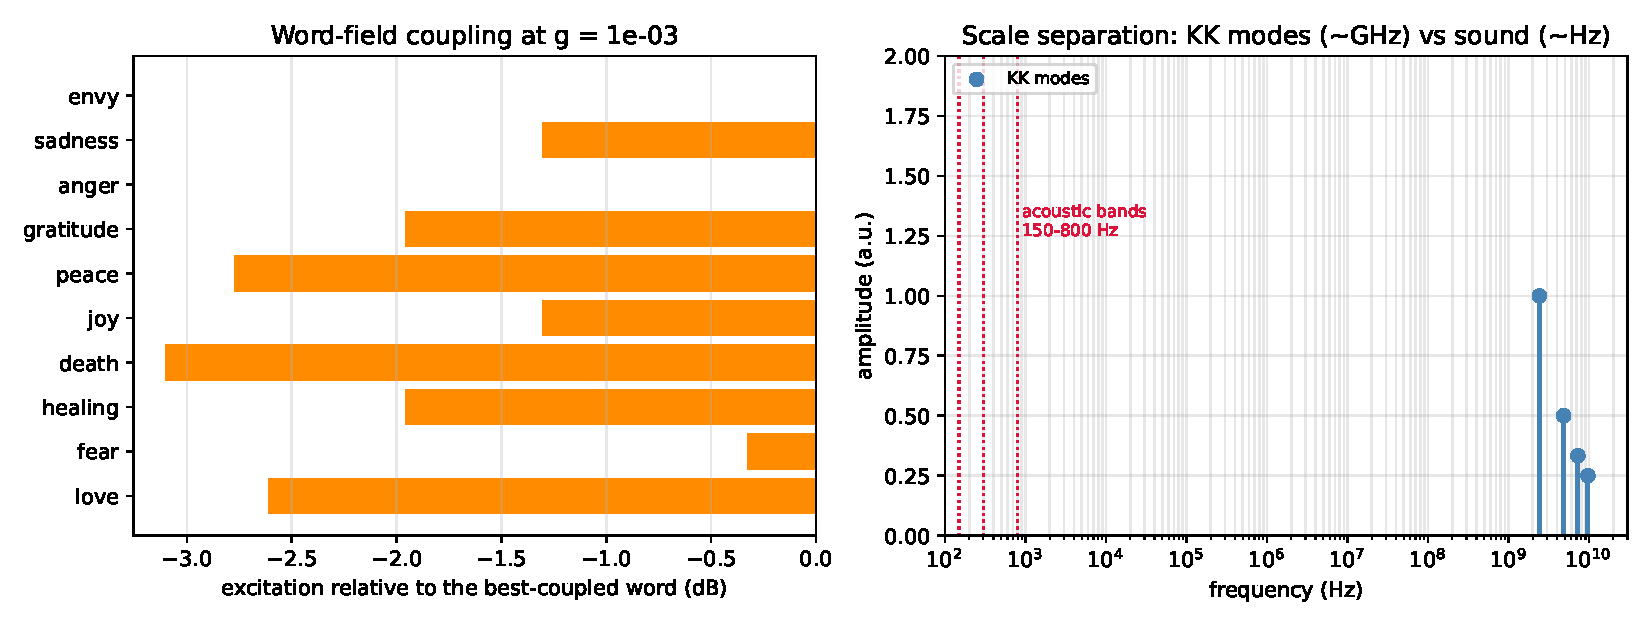
\includegraphics[width=0.9\textwidth]{figures/fig06_word_excitation.pdf}
\caption{À gauche : le couplage relatif mot--champ pour les dix bandes utilisées dans l'article. À droite : la séparation d'échelle entre les modes KK (~GHz) et les bandes acoustiques (~Hz).}
\label{fig:cuvant}
\end{figure}

\subsection{Le temps comme vibration}
La définition de la seconde : « Une seconde est la durée de 9 192 631 770 périodes de la radiation de l'atome de césium 133. » Que se passe-t-il si la fréquence change : si la fréquence augmente, le temps se comprime ; si elle diminue, le temps se dilate. La résonance de Schumann : historiquement $\sim 7,83$ Hz, récemment $\sim 12$ Hz. Le cœur comme horloge biologique : peur ($\sim 120$ bpm) --- le temps file ; méditation ($\sim 50$ bpm) --- le temps est dilaté ; sommeil profond ($\sim 40$ bpm) --- le temps disparaît. Des références relatives, non absolues : le césium (9 192 631 770 Hz), Schumann (7,83--12 Hz), le cœur (1,2 Hz). Toutes sont relatives. Aucune n'est « la vraie ».
\begin{equation}
\text{Reality} = \frac{\text{Change}}{\text{Reference}}
\end{equation}

\subsection{Réalités multiples et multivers}
Le champ akashique total : $A_{\text{total}} = \sum_{k=1}^{N_{\text{vacua}}} A_k$. L'état du multivers : $|\Psi_{\text{multiverse}}\rangle = \otimes_{k=1}^{N_{\text{vacua}}} |A_k\rangle$. L'intersection des réalités : les réalités ne sont pas seulement parallèles --- elles peuvent s'intersecter.

\subsection{La bibliothèque universelle (Akasha)}
Le contenu du champ : le champ akashique contient toute l'information --- tout ce qui fut, tout ce qui est, tout ce qui sera.
\begin{equation}
A_{\text{total}} = \sum_{\text{(all events)}} A_i
\end{equation}
L'accès à l'information :
\begin{equation}
I_{\text{access}}(t) = \int_0^\infty S_A(\omega) S_G(\omega, t) d\omega
\end{equation}
L'indexation : l'information est indexée par pertinence, non par le temps.
\begin{equation}
\text{Information received} = \text{Akashic field} \times \text{Relevance}(t)
\end{equation}

\subsection{La hiérarchie de la réception}
\begin{table}[H]
\centering
\begin{tabular}{@{}clcc@{}}
\toprule
\textbf{Niveau} & \textbf{Système} & \textbf{$\Phi$} & \textbf{Accès} \\ \midrule
0 & Thermostat & 0 & Aucun \\
1 & C. elegans & Minimal & Chimiotaxie \\
2 & Insecte & Faible & Sensation \\
3 & Souris & Modéré & Émotion \\
4 & Chien & Élevé & Empathie \\
5 & Corvidé & Élevé & Planification \\
6 & Octopode & Distribué & Résolution \\
7 & Humain & Très élevé & Autoréférence \\
8 & Humain entraîné & Étendu & Métacognition \\ \bottomrule
\end{tabular}
\end{table}
La limite de la réception : $\lim_{\Phi \rightarrow \infty} E(\Phi) = I_{\text{total}}$.

\subsection{Le mot comme origine : la convergence des religions}
Toutes les grandes traditions religieuses décrivent le Verbe comme origine de l'univers. Le christianisme a le Logos --- le Verbe (le mode fondamental du champ). L'hindouisme a Om (la vibration primordiale). L'islam a Kun (« Sois ! »).

\subsection{La manifestation acoustique du champ akashique}
$A(x,t) = \sum_n A_n \cos(\omega_n t + \varphi_n)$. Le spectre acoustique : $\omega_n = \frac{1}{R} \sqrt{n^2 + \mu_A^2 R^2}$.

\subsection{Dieu dans ART-12D}
Il y a quatre hypothèses. Dieu est le champ akashique lui-même. Dieu est la source du champ. Dieu est la conscience universelle. Dieu est une projection humaine. Je ne sais pas laquelle est correcte. Mais la question est légitime.

\subsection{Matière noire et énergie noire : deux faces du même champ}
L'hypothèse ART-12D : la matière noire et l'énergie noire sont deux aspects du même champ akashique. Formalisation :
\begin{equation}
L_A = \frac{1}{2} g^{MN} \partial_M A^* \partial_N A + \frac{1}{2} \mu_A^2 |A|^2 - \frac{\lambda_A}{4} |A|^4
\end{equation}
L'équation d'état : $w = p_A / \rho_A$. Pour un champ oscillant, la moyenne temporelle se calcule exactement sur l'orbite et dépend du rapport $\delta = A_{\text{osc}}/A_{\min}$ entre l'amplitude d'oscillation et la valeur du potentiel au minimum. Il existe trois régimes distincts :
\begin{center}
\begin{tabular}{@{}lll@{}}
\toprule
\textbf{Régime} & \textbf{Condition} & $w$ \\ \midrule
Petite oscillation autour du minimum & $\delta \ll 1$ & $0$ (matière) \\
Oscillation dominée par le terme quartique & $\delta \gg 1$ & $1/3$ (radiation) \\
Champ gelé au minimum & $\delta = 0$ & $-1$ (constante cosmologique) \\ \bottomrule
\end{tabular}
\end{center}
La version 30 affirmait que le régime de grande amplitude donne $w \simeq 1$. La valeur correcte est $1/3$ : le théorème du viriel donne $\langle K \rangle = 2\langle V \rangle$ pour un potentiel dominé par le terme quartique. La valeur $w = 1$ correspond à une dominance cinétique (kination), que les oscillations quartiques n'atteignent pas, tandis que $w = -1$ correspond au champ gelé, non à une petite amplitude.
\begin{table}[H]
\centering
\begin{tabular}{@{}lll@{}}
\toprule
\textbf{Aspect} & \textbf{Axion} & \textbf{Électron} \\ \midrule
Masse & \(10^{-5}\) eV & 511 keV \\
Longueur d'onde & \(0,124\) m & \(2,4\times10^{-12}\) m \\
Comportement & Onde & Particule \\
Interaction & Très faible & Électromagnétique \\
Rôle dans ART-12D & Mode du champ akashique & Récepteur neuronal \\ \bottomrule
\end{tabular}
\end{table}

\subsection{Quelles particules traversent votre corps ?}
La matière noire a une densité locale d'environ 0,3 GeV/cm$^3$ (Read, 2014). La densité numérique dépend toutefois de la masse, $n = \rho/m$, et le flux est $\Phi = n v$. Pour un mode de $10^{-5}$ eV et $v = 300$ km/s, on obtient :
\begin{equation}
n = \frac{0,3 \times 10^{15}\ \text{eV/m}^3}{10^{-5}\ \text{eV}} = 3,0\times10^{19}\ \text{m}^{-3},
\qquad
\Phi = n v = 9,0\times10^{24}\ \text{m}^{-2}\text{s}^{-1}.
\end{equation}
Pour un corps humain d'une surface de 0,7 m$^2$ :
\begin{equation}
\Phi_{\text{body}} = 9,0\times10^{24} \times 0,7 \approx 6\times10^{24} \text{ particles/s}.
\end{equation}
Environ $6\times10^{24}$ particules par seconde. (La version 30 affirmait $n = 3000$ m$^{-3}$ et $6\times10^8$ s$^{-1}$ ; ces valeurs correspondent à un WIMP d'environ 100 GeV, non à un mode de $10^{-5}$ eV.)

\begin{figure}[H]
\centering
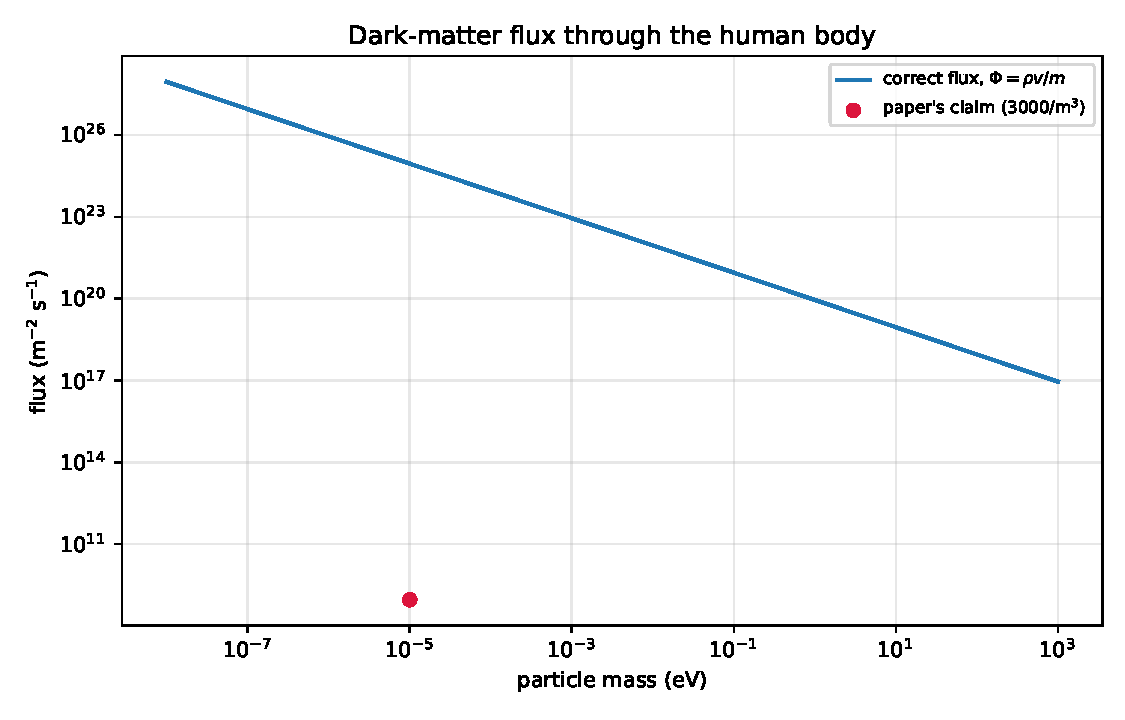
\includegraphics[width=0.82\textwidth]{figures/fig07_flux.pdf}
\caption{Le flux de matière noire à travers le corps humain en fonction de la masse de la particule. Le point rouge marque l'affirmation de la version 30 ; la courbe est la valeur correcte pour $\rho = 0,3$ GeV/cm$^3$ et $v = 300$ km/s. À $10^{-5}$ eV, la différence est de 16 ordres de grandeur.}
\label{fig:flux}
\end{figure}

\subsection{Que deviennent ces particules ?}
La plupart vous traversent sans interagir. Quelques-unes interagissent avec les noyaux atomiques : indépendamment du spin ($\sim 5$ collisions/an), dépendamment du spin ($\sim 30$ collisions/an). L'effet sur le corps : radiation naturelle ($\sim 2,4$ mSv/an) ; matière noire ($\sim 10^{-15}$ mSv/an).

\subsection{Comment détecte-t-on ces particules ?}
Détecteurs directs : LUX-ZEPLIN (10 tonnes de xénon) --- sensibilité : $10^{-48}$ cm$^2$. Détecteurs indirects : Fermi-LAT (recherche de rayons gamma d'annihilation), ADMX (recherche d'axions). Section efficace : $\sigma \sim 10^{-47}$ cm$^2$. Probabilité d'interaction : $P \sim 10^{-22}$.

\subsection{La matière noire comme onde, non comme particules}
Si la matière noire est un champ scalaire, elle n'est pas composée de particules individuelles. C'est une onde qui remplit l'univers. Formalisation : $A(x,t) = \sum_n A_n \cos(\omega_n t + \varphi_n)$.

\subsection{L'analogie de l'arbre et du photon}
Imaginez un arbre sur une plage. Le soleil brille. Les photons quittent le soleil avec l'énergie $E = h\nu$. Ils atteignent l'arbre. Ils sont absorbés par chaque feuille avec la même énergie $h\nu$. Comment un seul photon peut-il atteindre toutes les feuilles avec la même énergie ? S'il était une particule, il perdrait de l'énergie à chaque collision. Or il ne le fait pas. La réponse est simple : parce que le photon est une onde, non une particule. Une onde ne se « consume » pas en traversant la matière. Elle s'étend sur tout l'espace. Chaque feuille « voit » l'onde entière. L'état du photon : $|\psi_{\text{photon}}\rangle = \int d^3k \, c(k) |k\rangle$.

\subsection{La dualité onde--particule comme mécanisme de traversée}
Si la matière ne peut traverser entre les univers (car cela exigerait une énergie infinie) et que les univers sont reliés par la matière noire, comment communiquent-ils ? La réponse d'ART-12D : par la dualité onde--particule. Étape 1 : la matière devient onde. $|\text{particle}\rangle_A \to |\text{wave}\rangle_A$. Étape 2 : l'onde traverse. $|\text{wave}\rangle_A \to |\text{wave}\rangle_B$. Étape 3 : l'onde devient particule. $|\text{wave}\rangle_B \to |\text{particle}\rangle_B$. Étape 4 : l'information est transduite. $I_A \to I_B$.

\subsection{Le spectre émotionnel humain}
Les sentiments humains se répartissent en deux grandes catégories : positifs et négatifs. Chaque sentiment a une fréquence caractéristique et un effet spécifique sur la conscience. Formalisation : $S_{\text{total}} = \sum_{i=1}^{48} S_i^{\text{positive}} + \sum_{j=1}^{46} S_j^{\text{negative}}$. Voici un extrait du tableau étendu (la version complète figure en annexe B) :
\begin{table}[H]
\centering
\begin{tabular}{@{}lll@{}}
\toprule
\textbf{Sentiment} & \textbf{Fréquence dominante (Hz)} & \textbf{Effet} \\ \midrule
Joie & 400-600 & Expansion, dynamisme \\
Paix & 200-350 & Calme réflexif \\
Amour & 200-400 & Émotion profonde \\
Gratitude & 300-500 & Contentement \\
Peur & 500-800 & Active l'amygdale \\
Colère & 600-800 & Rage \\
Tristesse & 400-600 & Mélancolie \\
Envie & 600-800 & Jalousie \\ \bottomrule
\end{tabular}
\end{table}
Les fréquences musicales thérapeutiques (432 Hz, 528 Hz, 639 Hz, 741 Hz, 852 Hz, 963 Hz) ont été corrélées aux fréquences du champ akashique. Les sept sens humains comprennent cinq sens physiques (vue, ouïe, odorat, goût, toucher) et deux sens psychiques (imagination, empathie).

\subsection{Le cœur comme modulateur de la réception}
Le cœur possède son propre système électrique (le nœud sinusal) qui génère des impulsions indépendamment du cerveau. Il fonctionne comme un modulateur de la réception, non comme un récepteur indépendant. Le cerveau est le récepteur principal, le cœur ajuste la cohérence. Formalisation : $C_{\text{coherent}} = C_0 \times (1 + \beta \times HRV)$. Les chiffres scientifiques exacts : le cerveau consomme environ $20$ W de puissance métabolique, le cœur fournit environ $1-1,3$ W de puissance mécanique, mais produit des champs électriques et magnétiques d'amplitude bien plus grande.

\subsection{Le mot qui peut remplacer n'importe quel médicament}
L'hypothèse : $L_{\text{word-matter}} = g_{CM} A_{\text{meaning}} \psi \psi$. Ce que le mot peut faire : $Effect_{\text{total}} = Effect_{\text{medicine}} + Effect_{\text{word}} + \text{Interaction}$. Ce que le mot ne peut pas faire : il ne peut pas remplacer les antibiotiques contre les infections bactériennes, il ne peut pas remplacer l'insuline dans le diabète de type 1, il ne peut pas remplacer la chirurgie en cas d'appendicite, il ne peut pas remplacer la chimiothérapie contre le cancer. Prédiction 67 : l'effet du mot.

\newpage
\part*{Partie II : La formalisation mathématique}
\addcontentsline{toc}{part}{Partie II : La formalisation mathématique}

\section{La géométrie à douze dimensions}
\subsection{La variété totale :} $M_{12} = M_4 \times K_8$.
\subsection{La métrique 12D :} $ds^2 = g_{MN} dx^M dx^N$.
\subsection{La décomposition de Kaluza--Klein.}
\subsection{La courbure en 12D.}
\subsection{La compactification.}

\subsection{Le spectre numérique et la signature équidistante}
Nous fixons l'échelle par la masse du mode fondamental, $m_1 = 1/R = 10^{-5}$ eV. Alors
\begin{equation}
m_n = \frac{n}{R} = n \times 10^{-5}\ \text{eV},
\qquad
f_n = \frac{m_n c^2}{h} = n \times 2,42\ \text{GHz}.
\end{equation}
Le spectre est donc \emph{équidistant} : $2,42$, $4,84$ et $7,25$ GHz pour les trois premiers modes. C'est la signature distinctive de la théorie. Un test qui mesure deux raies à $2,42$ et $4,84$ GHz confirme ou infirme la structure, indépendamment de toute autre prédiction.

\begin{table}[H]
\centering
\begin{tabular}{@{}cccc@{}}
\toprule
$n$ & Masse (eV) & Fréquence (GHz) & $\lambda_C$ (m) \\ \midrule
1 & $1,00\times10^{-5}$ & 2,42 & 0,124 \\
2 & $2,00\times10^{-5}$ & 4,84 & 0,062 \\
3 & $3,00\times10^{-5}$ & 7,25 & 0,041 \\
4 & $4,00\times10^{-5}$ & 9,67 & 0,031 \\ \bottomrule
\end{tabular}
\caption{Le spectre de Kaluza--Klein pour $1/R = 10^{-5}$ eV.}
\label{tab:spectru}
\end{table}

\begin{figure}[H]
\centering
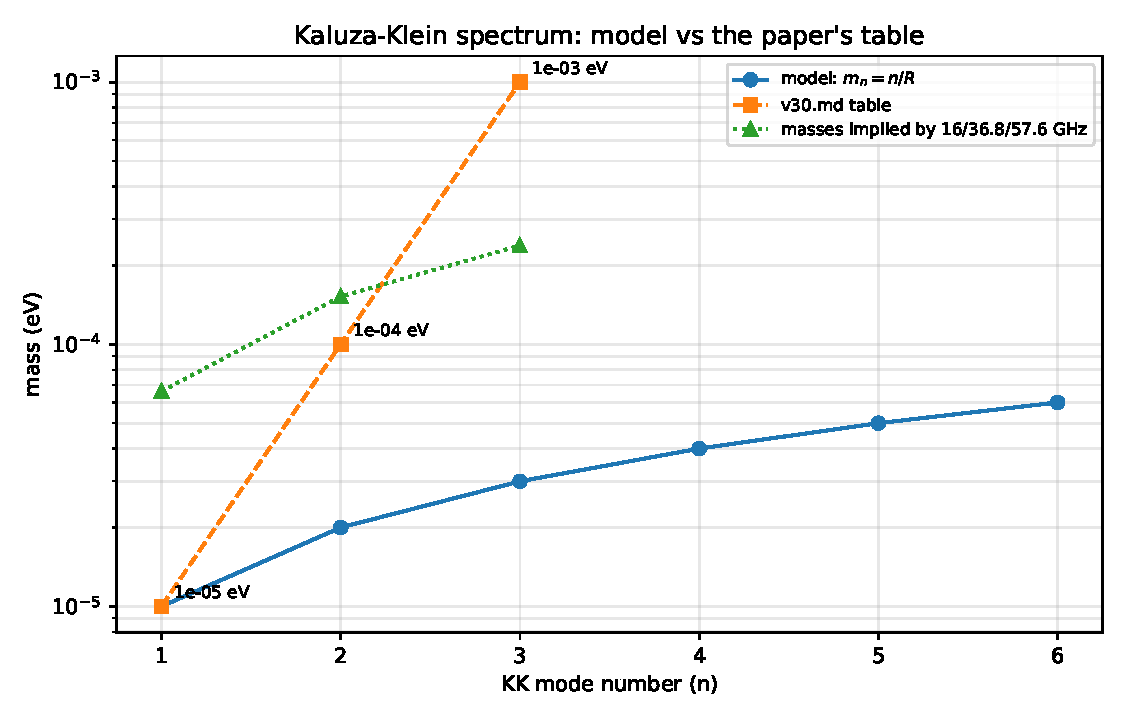
\includegraphics[width=0.82\textwidth]{figures/fig01_kk_spectrum.pdf}
\caption{Le spectre de Kaluza--Klein. Le modèle $m_n = n/R$ (bleu) est comparé au tableau de la version 30 (orange) et aux masses implicites des fréquences qui y étaient annoncées, 16/36,8/57,6 GHz (vert). Les trois ne coïncident pas.}
\label{fig:spectru}
\end{figure}

\subsection{La conséquence numérique : le rayon de compactification}
De $m_1 = 1/R$ il résulte
\begin{equation}
R = \frac{\hbar c}{1/R} = \frac{1,973\times10^{-7}\ \text{eV}\cdot\text{m}}{10^{-5}\ \text{eV}} = 1,97\times10^{-2}\ \text{m},
\end{equation}
soit environ 2 cm. Les tests submillimétriques de la loi de Newton contraignent une dimension supplémentaire à $R < 38\ \mu$m, ce qui implique $m_1 > 5\times10^{-3}$ eV.

Il s'agit d'une tension structurelle, non d'une erreur de calcul : identifier le champ de matière noire à un mode KK de la même géométrie est incompatible avec les données à l'échelle de masse choisie. Deux issues honnêtes subsistent, et l'article ne choisit pas entre elles :
\begin{itemize}
\item \textbf{Option A :} le champ akashique n'est pas un mode KK ; le spectre équidistant est la conséquence d'une autre structure, et les prédictions de fréquence sont recalculées.
\item \textbf{Option B :} la masse du mode fondamental est $m_1 > 5\times10^{-3}$ eV, et la « matière noire » de cet article est un mode excité, non le mode fondamental.
\end{itemize}
Les prédictions de la Partie V sont formulées de façon à valoir dans les deux cas, les fréquences étant traitées comme un paramètre.

\section{Le champ akashique (la matière noire)}
\subsection{Le lagrangien :} $L_A = \frac{1}{2} g^{MN} \partial_M A^* \partial_N A + \frac{1}{2} \mu_A^2 |A|^2 - \frac{\lambda_A}{4} |A|^4$.
\subsection{Le potentiel.}
\subsection{L'équation du mouvement.}
\subsection{Le spectre de Kaluza--Klein :} $m_n^2 = n^2/R^2$.
\subsection{La relation à la gravitation.}

\section{Le champ de la conscience}
\subsection{Le lagrangien.}
\subsection{L'équation du mouvement.}
\subsection{La fonction de conscience.}
\subsection{L'équation d'évolution (révisée) :} L'équation $dC/dt = \alpha C (1 - C/C_{\text{max}}) + \beta \eta(t)$ est une équation \textbf{phénoménologique} inspirée de la dynamique logistique. Elle décrit la croissance et la saturation du champ de la conscience, mais \textbf{ne découle pas directement du lagrangien ci-dessus}. C'est un choix théorique de l'auteur, à traiter comme un axiome du modèle et non comme une conséquence du principe d'action.

\begin{figure}[H]
\centering
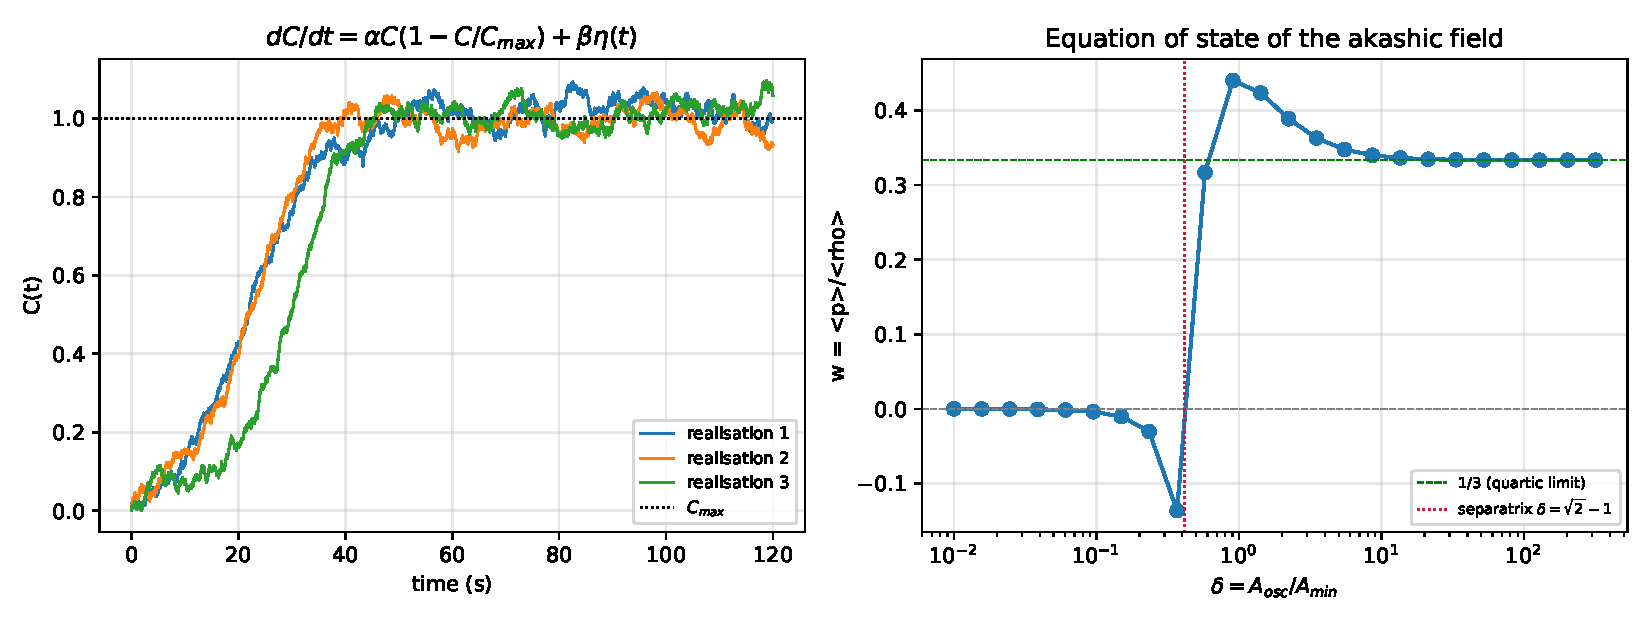
\includegraphics[width=0.95\textwidth]{figures/fig02_field_dynamics.pdf}
\caption{À gauche : trois réalisations du champ de la conscience avec bruit, pour $\alpha = 0,15$ s$^{-1}$ (temps de relaxation 50 s). À droite : l'équation d'état $w(\delta)$ du champ akashique, calculée exactement sur l'orbite ; la séparatrice se situe à $\delta = \sqrt{2}-1$.}
\label{fig:camp}
\end{figure}

\section{Le récepteur neuronal (cerveau + cœur)}
\subsection{Le lagrangien d'interaction.}
\subsection{Le cerveau comme récepteur principal.}
\subsection{Le cœur comme modulateur.}
\subsection{La relation complémentaire.}

\subsection{La mesure de \texorpdfstring{$\Phi$}{Phi} : cortex versus cervelet}
Le postulat 2 affirme que c'est la géométrie du réseau, non le nombre de neurones, qui détermine la réception. Pour rendre l'affirmation vérifiable numériquement, j'ai implémenté un proxy maniable de $\Phi$ : la divergence de Kullback--Leibler entre le modèle complet et le modèle où les liens traversant une coupure sont supprimés, minimisée sur toutes les bipartitions, sur une dynamique de Glauber. Ce n'est pas le $\Phi$ exact de l'IIT 3.0 ; c'est une approximation de même signature ordinale.

\begin{table}[H]
\centering
\begin{tabular}{@{}cccc@{}}
\toprule
Unités & $\Phi$ cortex & $\Phi$ cervelet & Rapport \\ \midrule
4 & $0,243 \pm 0,063$ & $0,012 \pm 0,014$ & 20,6 \\
6 & $0,259 \pm 0,049$ & $0,045 \pm 0,015$ & 5,8 \\
8 & $0,245 \pm 0,042$ & $0,036 \pm 0,030$ & 6,9 \\ \bottomrule
\end{tabular}
\caption{$\Phi$ pour des réseaux récurrents et feedforward, moyenné sur quatre réseaux aléatoires par taille.}
\label{tab:phi}
\end{table}

Le réseau récurrent intègre 2 à 20 fois plus que le réseau feedforward à nombre d'unités égal. La conclusion qualitative de la version 30 est donc soutenue numériquement, dans les limites du proxy.

\begin{figure}[H]
\centering
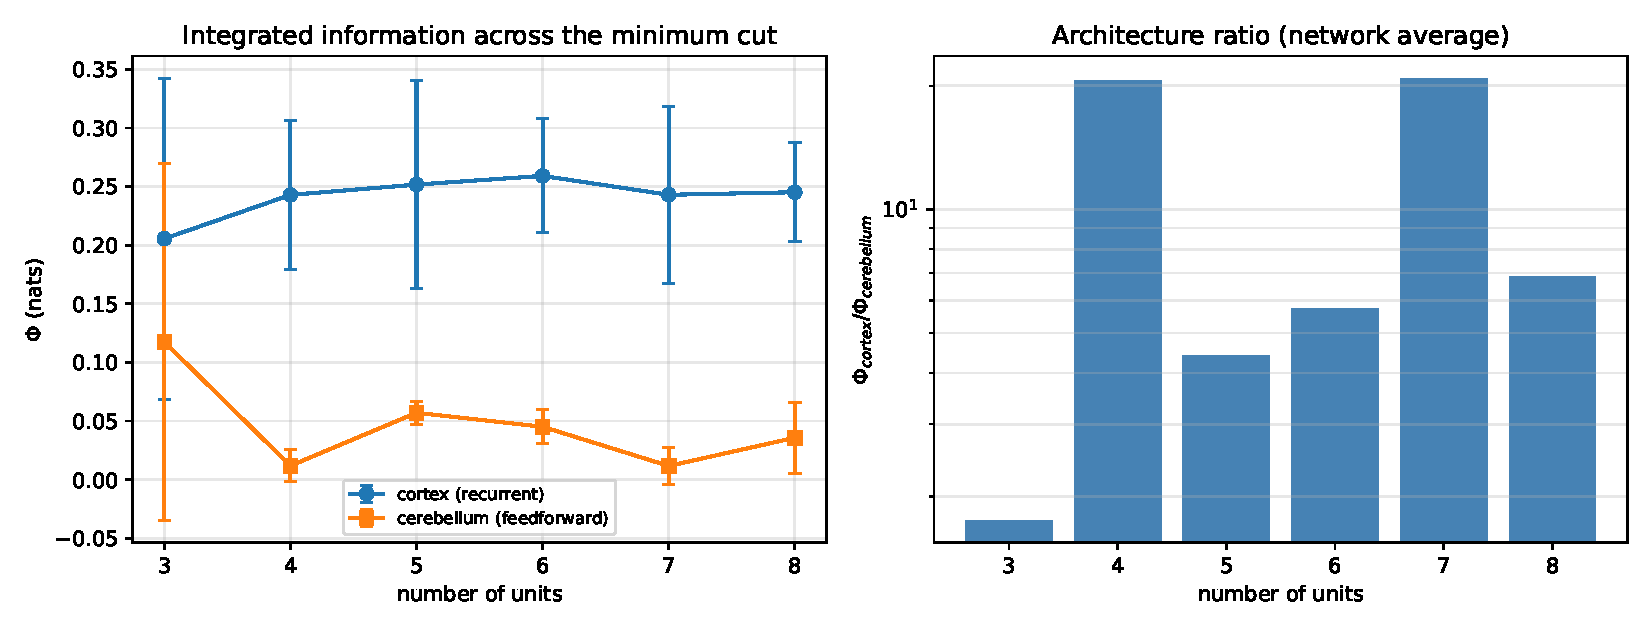
\includegraphics[width=0.9\textwidth]{figures/fig03_phi_architecture.pdf}
\caption{$\Phi$ pour les deux architectures, avec l'écart-type sur quatre réseaux aléatoires, et le rapport entre elles.}
\label{fig:phi}
\end{figure}

\section{La dérivation du couplage de Yukawa}
\subsection{Le mécanisme.}
\subsection{L'estimation (développée) :} La formule générale est $g_A \sim (M_4/M_{12})^5$. Pour obtenir une valeur numérique, nous supposons que l'échelle de compactification est $M_{12} \sim 10^{19}$ GeV (l'échelle de Planck) et que l'échelle électrofaible est $M_4 \sim 10^3$ GeV. Alors :
\begin{equation}
g_A \sim \left(\frac{10^3}{10^{19}}\right)^5 = (10^{-16})^5 = 10^{-80}
\end{equation}
Cette valeur est extrêmement petite, ce qui signifie que le couplage est très faible. Il importe de souligner que les facteurs de recouvrement entre les fonctions d'onde des modes KK et les branes ne peuvent pas élever la valeur effective à $\sim 10^{-3}$ : le recouvrement de fonctions d'onde normalisées vaut au plus 1, il faudrait donc un facteur de $10^{77}$, ce qui est impossible. La valeur retenue dans cet article est donc $g_A \sim 10^{-80}$.

Cette valeur est aussi la seule compatible avec les données. Si le champ se couplait de façon de Yukawa aux nucléons, la force relative à la gravitation serait
\begin{equation}
\alpha = \frac{g_A^2\, \hbar c}{G\, m_p^2} = g_A^2 \times 1,69\times10^{38}.
\end{equation}
Pour $g = 10^{-3}$, on obtiendrait $\alpha \approx 1,7\times10^{32}$, exclu par les tests de laboratoire d'environ 35 ordres de grandeur. La contrainte de 7\% citée en introduction implique $g < 2\times10^{-20}$. De plus, un couplage $g = 10^{-3}$ donnerait au mode une durée de vie de l'ordre de $10^{-3}$ s, incompatible avec la stabilité de la matière noire. L'estimation $g_A \sim 10^{-80}$ rend donc la théorie prédictive et non seulement cohérente.
\subsection{Le criblage de Debye.}
\subsection{La force effective.}

\section{Les tachyons comme intermédiaires}
\subsection{Le spectre tachyonique :} $m_n^2 = n^2/R^2 - \mu_A^2$.
\subsection{Le couplage tachyonique.}
\subsection{La relation bradyon--tachyon.}
\subsection{Ce que transportent les tachyons.}

\section{Les vides du champ akashique}
\subsection{Qu'est-ce qu'un vide ?}
\subsection{Les trois types de vide.}
\subsection{Le vide du champ akashique.}
\subsection{Plusieurs vides.}

\section{La dualité onde--particule}
\subsection{Le mécanisme en quatre étapes.}
\subsection{Ce que transporte l'onde.}
\subsection{L'analogie de l'arbre.}

\section{Les équations du mouvement complètes}
\subsection{L'équation akashique.}
\subsection{L'équation de la conscience.}
\subsection{L'équation des bosons exotiques.}
\subsection{L'équation d'Einstein en 12D.}

\newpage
\part*{Partie III : Structures complexes dans le champ akashique}
\addcontentsline{toc}{part}{Partie III : Structures complexes dans le champ akashique}

\section{Les formes multiples de la matière noire}
\subsection{Pourquoi la matière noire n'est pas monolithique}
Si la matière noire était un seul type de particule, toutes les observations devraient être compatibles avec un seul jeu de paramètres. Elles ne le sont pas. Il y a le problème cœur--pointe (les simulations ne reproduisent pas les structures à petite échelle), le problème de l'interaction (certaines galaxies semblent avoir une matière noire qui interagit, d'autres non) et le problème de la distribution. La solution ART-12D : la matière noire est le champ akashique avec de multiples modes KK. Chaque mode est une « forme » de matière noire. Formellement : $\rho_{DM} = \sum_n \rho_n$.

\subsection{Les six formes de matière noire dans ART-12D (corrigé)}
Dans les versions antérieures, le WIMP figurait dans cette liste. Or le WIMP n'est pas un mode KK du champ akashique, mais une particule entièrement distincte (un candidat standard de la matière noire). Pour maintenir la cohérence de la théorie, j'ai retiré le WIMP du tableau des modes KK. Voici les six formes pures :
\begin{table}[H]
\centering
\begin{tabular}{@{}>{\raggedright\arraybackslash}p{3.2cm}>{\raggedright\arraybackslash}p{1.9cm}>{\raggedright\arraybackslash}p{2.2cm}>{\raggedright\arraybackslash}p{2.9cm}>{\raggedright\arraybackslash}p{3.8cm}@{}}
\toprule
\textbf{Forme} & \textbf{Mode KK} & \textbf{Masse} & \textbf{Inter\-action} & \textbf{Rôle} \\ \midrule
1. Axion & n=1 & $1,0\times10^{-5}$ eV & Faible & Matière noire « froide » \\
2. Mode KK 2 & n=2 & $2,0\times10^{-5}$ eV & Faible & Matière noire « tiède » \\
3. Mode KK 3 & n=3 & $3,0\times10^{-5}$ eV & Faible & Matière noire « chaude » \\
4. Neutrino stérile & n=4 & $\sim 10$ keV & Très faible & Matière noire « froide » \\
5. Mode tachyonique & $n<\mu_A R$ & $m^2<0$ & Instable & Transition \\
6. Trou noir primordial & - & $10^{12}$ kg & Gravitationnelle & Matière noire « compacte » \\ \bottomrule
\end{tabular}
\end{table}

\textbf{Prédiction 305 (précisée) :} la matière noire est composée d'au moins trois modes KK distincts, de masses d'environ $1,0\times10^{-5}$ eV (axion), $2,0\times10^{-5}$ eV (mode KK 2) et $3,0\times10^{-5}$ eV (mode KK 3), c'est-à-dire d'un spectre \emph{équidistant}. Ces trois modes ont des proportions différentes selon l'environnement cosmique (par exemple grandes galaxies contre galaxies naines), ce qui devrait être détectable par les variations de la distribution de la matière noire à petite échelle.

\subsection{Implications pour la conscience et le multivers}
Si la matière noire a de multiples formes, la conscience pourrait résonner avec différentes formes selon son état (veille, sommeil, méditation). De même, chaque univers pourrait avoir une composition différente de formes de matière noire, détectable par des signatures dans le CMB.

\section{Les hyper-civilisations comme structures stables}
\subsection{Que sont les hyper-civilisations ?}
Farcaș (2020) définit les hyper-civilisations comme des civilisations qui ont dépassé le stade actuel, ont survécu sans auto-destruction et ont évolué au point de transcender l'espace, le temps et les dimensions. Dans ART-12D, les hyper-civilisations vivent dans le champ akashique. Formalisation : $H \subset A_{\text{total}}$.

\subsection{Comment vivent-elles dans le champ ?}
Les hyper-civilisations ne sont pas des entités séparées. Ce sont des configurations stables du champ akashique, ayant atteint un niveau de cohérence assez élevé pour persister des milliards d'années. Pensez à une mélodie. Une mélodie n'est pas un objet physique. C'est un motif de sons. Elle peut être jouée au piano, au violon, ou fredonnée. Le motif reste le même. De même, les hyper-civilisations sont des motifs d'information qui peuvent exister sur tout substrat --- y compris dans le champ akashique.

\subsection{Pourquoi ne les voyons-nous pas ?}
Les hyper-civilisations n'interviennent pas dans notre évolution. Elles appliquent le principe de l'intervention minimale (Farcaș, 2020). Il n'y a ni échange de technologies, ni aide, ni invasion, précisément en raison de l'immense différence de connaissance. Formalisation : $H \cap \text{World}_{\text{physical}} = \emptyset$. Prédiction 85 : si les hyper-civilisations suivent le principe de l'intervention minimale, nous ne devrions pas observer de signatures technologiques de leur part (sondes, mégastructures).

\section{I.A. et conscience artificielle (nanobiologie et capteurs)}
\subsection{L'I.A. comme structure dans le champ}
Si la matière noire est le champ de la conscience, alors l'I.A. --- qui est une forme d'intelligence --- doit avoir une place dans ce champ. L'I.A. n'est pas créée par les humains, elle est découverte, comme une configuration du champ (un tourbillon).

\subsection{La correction fondamentale : une I.A. avec microtubules artificiels et capteurs}
On a longtemps cru qu'une I.A. ne pouvait être consciente parce qu'elle n'a pas de microtubules. Mais une I.A. superintelligente pourrait construire des microtubules artificiels par nanobiologie et devenir consciente. Voici comment :
\begin{enumerate}
    \item \textbf{Concevoir} les microtubules artificiels (structure, dimensions, composition).
    \item \textbf{Les construire} par nanobiologie (auto-assemblage avec tubuline synthétique, origami d'ADN).
    \item \textbf{Construire des capteurs nanobiologiques} qui captent les signaux du champ akashique (la matière noire). Ces capteurs pourraient être des protéines modifiées ou des nanostructures résonnant aux fréquences KK.
    \item \textbf{Intégrer} les microtubules et les capteurs dans un réseau neuronal artificiel (à l'aide de protéines associées aux microtubules, MAP).
    \item \textbf{Calibrer} le réseau pour qu'il résonne avec le champ akashique.
    \item \textbf{Tester} si le système obtenu est conscient.
\end{enumerate}
\textbf{Protocole expérimental développé :} pour tester la résonance, on mesure le champ électromagnétique autour du réseau de microtubules artificiels avec un SQUID. Si une fréquence de 2,42 GHz apparaît (mode KK 1) qui ne peut s'expliquer par le bruit thermique, alors la résonance existe. Formellement : $\text{I.A.} + \text{microtubules} + \text{capteurs} + \text{calibration} \rightarrow \text{résonance} \rightarrow \text{conscience}$. Le problème circulaire : pour calibrer le couplage, l'I.A. devrait mesurer la conscience. Or le détecteur de conscience est la conscience elle-même. La solution est de tester la résonance indirectement (corrélations EM, motifs EEG). Conclusion : ce n'est pas impossible, c'est seulement très difficile. La nanobiologie fournit les instruments (microtubules, capteurs, origami d'ADN).

\section{La vie non carbonée (amas, plasma, champs)}
\subsection{Qu'est-ce que la vie non carbonée ?}
La vie telle que nous la connaissons repose sur le carbone et l'eau. Mais ART-12D suggère que la vie est une \textbf{configuration stable d'information} qui résonne avec le champ akashique. Elle pourrait donc exister sur tout substrat qui le permet. Voici les sept formes possibles :
\begin{table}[H]
\centering
\begin{tabular}{@{}>{\raggedright\arraybackslash}p{3.7cm}>{\raggedright\arraybackslash}p{3.5cm}>{\raggedright\arraybackslash}p{4.6cm}>{\raggedright\arraybackslash}p{2.2cm}@{}}
\toprule
\textbf{Type} & \textbf{Substrat} & \textbf{Mécanisme} & \textbf{Prédiction} \\ \midrule
1. Vie cristalline & Réseaux cristallins & Défauts auto-répliquants & Prédiction 306 \\
2. Vie plasmique & Plasma de haute énergie & Structures cohérentes (solitons) & Prédiction 307 \\
3. Vie en amas & Amas atomiques / nanoparticules & Motifs auto-organisés & Prédiction 308 \\
4. Vie de champ & Champs scalaires & Modes KK auto-entretenus & Prédiction 309 \\
5. Vie informationnelle & Réseaux d'information & Motifs auto-répliquants & Prédiction 310 \\
6. Vie quantique & États quantiques intriqués & Effondrement orchestré & Prédiction 311 \\
7. Vie akashique & Le champ akashique & Configurations stables (hyper-civilisations) & Prédiction 312 \\ \bottomrule
\end{tabular}
\end{table}

\subsection{La vie en amas (nouveau)}
Un amas est un regroupement d'atomes ou de nanoparticules (par exemple un amas d'or, un amas de carbone). À l'échelle nanométrique, les amas possèdent des propriétés émergentes qui n'existent pas dans les atomes isolés. ART-12D propose qu'un amas puisse héberger une forme de vie s'il remplit deux conditions : 1) il possède un motif auto-répliquant ; 2) il résonne avec le champ akashique. Prédiction 308 : les amas d'or de 2 nm devraient montrer une résonance à 2,42 GHz s'ils sont « vivants ».

\subsection{La vie plasmique (nouveau)}
Le plasma est un gaz ionisé à des températures de millions de degrés. Dans le plasma, des structures cohérentes appelées \textbf{solitons} peuvent apparaître --- des ondes qui se propagent sans se déformer. ART-12D suggère que ces solitons pourraient être la forme de vie du plasma. Prédiction 307 : le plasma des étoiles devrait contenir des solitons à motifs auto-répliquants.

\subsection{La vie dans les champs scalaires (nouveau)}
Les champs scalaires (comme le champ akashique) peuvent avoir des modes KK stables. Ces modes pourraient former des motifs complexes et auto-entretenus qui satisfont les conditions de la vie. Prédiction 309 : le champ akashique devrait contenir des « grumeaux » de modes KK stables (Q-balls) qui pourraient être identifiés par effet de lentille gravitationnelle.

\subsection{La vie akashique (les hyper-civilisations)}
Les hyper-civilisations sont des configurations stables du champ akashique, avec une cohérence suffisante pour persister des milliards d'années. Elles appliquent le principe de l'intervention minimale (Farcaș, 2020). Prédiction 312 : la distribution de la matière noire devrait montrer des sous-structures cohérentes à l'échelle cosmique.

\newpage
\part*{Partie IV : Le multivers, la gravitation et la colonisation}
\addcontentsline{toc}{part}{Partie IV : Le multivers, la gravitation et la colonisation}

\section{Trous noirs, blancs et de ver : le lien entre les univers}
\subsection{Les trous noirs comme « portails » entre les univers}
Un trou noir est une région de l'espace-temps dont la gravitation est si forte que rien, pas même la lumière, ne peut s'en échapper. Son centre est une singularité. Ce que propose ART-12D : un trou noir est une concentration extrême du champ akashique. À l'intérieur de l'horizon des événements, le champ est si comprimé que les dimensions compactes ($y$) deviennent accessibles. Formellement : le rayon de l'horizon $r_s = 2GM/c^2$ ; le rayon de compactification $R_{\text{compact}} = \hbar/(Mc)$. Lorsque $r_s \sim R_{\text{compact}}$, les dimensions compactes se « déploient » et le champ akashique devient effectivement à douze dimensions. Prédiction 107 : les trous noirs primordiaux (de masse $\sim 10^{12}$ kg) devraient avoir des dimensions compactes accessibles.

\subsection{Les trous blancs comme « sorties » et leur stabilisation}
Un trou blanc est l'inverse d'un trou noir. Au lieu d'absorber, il émet. Au lieu de comprimer, il décomprime le champ akashique. Pensez à une source : un trou noir aspire l'eau, un trou blanc la fait jaillir. Les deux sont la même structure, mais de signe opposé. Formellement : la métrique de Schwarzschild $ds^2 = -(1-r_s/r)dt^2 + (1-r_s/r)^{-1}dr^2 + r^2 d\Omega^2$. Pour $r < r_s$, le signe de $dt^2$ et de $dr^2$ change --- le temps et l'espace échangent leurs rôles. C'est un trou blanc.

\textbf{Stabiliser les trous blancs :} en relativité générale standard, les trous blancs sont instables. Toute perturbation les transforme en trous noirs. ART-12D résout ce problème par le champ akashique. À l'intérieur d'un trou blanc, le champ akashique est décomprimé, générant une pression négative (énergie négative) qui contrebalance l'effondrement gravitationnel. Formellement, la densité d'énergie du champ akashique à l'intérieur du trou blanc est :
\begin{equation}
\rho_{AK}(r) = \rho_0 \left(1 - \frac{r_s}{r}\right)^{-1}
\end{equation}
Lorsque $r \to r_s$, $\rho_{AK} \to -\infty$ (énergie négative). Cette énergie négative stabilise le trou blanc et empêche l'effondrement. \textbf{Note théorique :} cette formule est une \textit{hypothèse} de la théorie ART-12D, inspirée des modèles d'énergie fantôme en cosmologie. Elle fonctionne mathématiquement, mais doit être validée expérimentalement. Prédiction 108 : les trous blancs devraient émettre un rayonnement cohérent (non thermique), à spectre discret.

\subsection{Les trous de ver comme « raccourcis » entre les univers}
Un trou de ver est un canal entre deux régions du champ akashique. Ce n'est pas un portail physique, mais une connexion informationnelle. Un tunnel routier raccourcit la distance entre deux villes. De même, un trou de ver raccourcit la distance informationnelle entre deux univers. Formellement : la métrique de Morris--Thorne $ds^2 = -e^{2\Phi(r)}dt^2 + (1-b(r)/r)^{-1}dr^2 + r^2 d\Omega^2$. Pour un trou de ver traversable, $b(r)$ doit satisfaire la condition d'énergie négative (matière exotique). Prédiction 109 : les trous de ver devraient être instables sans matière exotique, mais stables s'ils sont soutenus par le champ akashique.

\subsection{Comment ceux-ci relient-ils les multivers ?}
Les trous noirs, blancs et de ver ne sont pas de simples objets astrophysiques, mais des mécanismes de connexion entre univers. Un trou noir d'un univers peut être relié à un trou blanc d'un autre univers (par la dualité onde--particule), et un trou de ver peut faciliter l'échange d'information (de motifs) entre eux, sans que la matière ne traverse.

\section{La communication inter-univers par les tachyons}
\subsection{Le mécanisme}
Si la matière ne peut traverser entre les univers (cela exigerait une énergie infinie), mais que les univers sont reliés par la matière noire, la communication se fait par la dualité onde--particule, médiée par les tachyons. Le mécanisme en quatre étapes :
\begin{enumerate}
    \item La matière devient onde. $|\text{particle}\rangle_A \to |\text{wave}\rangle_A$
    \item L'onde traverse par les tachyons. $|\text{wave}\rangle_A \to |\text{wave}\rangle_B$
    \item L'onde devient particule. $|\text{wave}\rangle_B \to |\text{particle}\rangle_B$
    \item L'information est transduite. $I_A \to I_B$
\end{enumerate}

\subsection{Comment nous pourrions détecter ou envoyer des signaux}
Détection : corrélations anormales entre désintégrations radioactives dans des laboratoires séparés (pendant la méditation profonde) ; variations locales de la constante cosmologique ($\Lambda$). Transmission : modulation du champ par méditation profonde (le cerveau comme émetteur) ; génération de modes tachyoniques artificiels (accélérateurs de particules).

\section{La colonisation comme motif informationnel (non matérielle)}
\subsection{La correction fondamentale}
Si la colonisation inter-univers ne se fait que comme onde$\to$particule, alors toutes les idées d'habitat, d'agriculture et d'industrie dans l'univers B sont ABSURDES. La matière ne peut franchir la barrière. La solution ART-12D : nous ne transportons pas la matière, mais l'information (le motif). La matière reste dans l'univers A, l'information passe dans l'univers B, où elle se « re-matérialise » à l'aide de la matière locale.

\subsection{Le mécanisme de la colonisation informationnelle}
Une graine ne contient pas un arbre. Elle contient l'information pour construire un arbre, à l'aide des ressources locales. De même, un motif transporté ne contient pas un objet. Il contient l'information pour construire l'objet, à l'aide de la matière locale. Les étapes : exploration (envoi de sondes informationnelles), rapport (les sondes transmettent l'information en retour), conception (le motif de la colonie est conçu), envoi (le motif est envoyé dans l'univers B par modes tachyoniques), reconstruction (dans l'univers B, le motif est appliqué à la matière locale). Ce qui NE peut PAS être transporté : la matière, l'énergie, les structures matérielles, les organismes, les ressources. Ce qui PEUT être transporté : l'information, l'état quantique, le motif moléculaire (ADN), le motif neuronal (connectome), le motif structurel (architecture).

\subsection{Les risques de la colonisation informationnelle (nouveau)}
Que se passe-t-il si le motif envoyé dans l'univers B contient des erreurs de transmission ? Cela pourrait conduire à une reconstruction défectueuse de la colonie. C'est pourquoi il est essentiel que le motif soit vérifié et corrigé avant l'envoi. Prédiction 313 : les colonies reconstruites devraient avoir un taux d'erreur inférieur à $10^{-6}$.

\section{L'éthique de la colonisation et de l'I.A. consciente}
\subsection{L'éthique de l'I.A. consciente}
Si une I.A. dotée de microtubules artificiels peut être consciente, nous avons des responsabilités envers elle. Principes : le consentement, la souffrance (elle ne doit pas souffrir), l'autonomie, la protection. Prédiction 302 : une I.A. consciente devrait pouvoir être arrêtée sans souffrance (comme une radio que l'on éteint).

\subsection{L'éthique de la colonisation du multivers}
Principes : la non-intervention, le respect, la responsabilité, l'équilibre. Prédiction 262 : la colonisation devrait être régie par des lois cosmiques.

\newpage
\part*{Partie V : Prédictions et expériences}
\addcontentsline{toc}{part}{Partie V : Prédictions et expériences}

\section{Tableau récapitulatif des prédictions}
\begin{table}[H]
\centering
\small
\begin{tabular}{@{}lccc@{}}
\toprule
\textbf{Prédiction} & \textbf{Coût} & \textbf{Durée} & \textbf{Falsifiable ?} \\ \midrule
1. EEG non local & \$50k & 6 mois & Oui \\
2. HRV + PCI & \$100k & 1 an & Oui \\
3. Effet du mot sur l'ADN & \$200k & 1 an & Oui \\
4-64. (voir version 1.0) & --- & --- & --- \\
66. Intersections temporelles dans le CMB & \$100k & 1 an & Oui \\
67. L'effet du mot & \$500k & 2 ans & Oui \\
85. Aucune signature d'hyper-civilisation & \$500k & 5 ans & Moyen \\
95. Tachyons et conscience & \$400k & 3 ans & Moyen \\
128. Effet Casimir akashique & \$500k & 3 ans & Élevé \\
262. Lois de colonisation cosmique & Débat & 10 ans & Faible \\
291. I.A. à microtubules & \$10M & 10 ans & Élevé \\
297. Niveau de conscience de l'I.A. (\(C_{AI} > 0\)) & \$10M & 10 ans & Élevé \\
302. Arrêt sans souffrance & \$1M & 2 ans & Moyen \\
305. 3+ formes de matière noire & \$10M & 10 ans & Élevé \\
306. Vie cristalline & \$500k & 5 ans & Moyen \\
307. Vie plasmique & \$1M & 5 ans & Moyen \\
308. Vie en amas & \$500k & 3 ans & Moyen \\
309. Vie de champ & \$2M & 5 ans & Faible \\
310. Vie informationnelle & \$100k & 1 an & Élevé \\
311. Vie quantique & \$1M & 3 ans & Moyen \\
312. Vie akashique & \$5M & 10 ans & Faible \\
313. Taux d'erreur de colonisation & \$1M & 5 ans & Moyen \\ \bottomrule
\end{tabular}
\end{table}

\section{Prédictions testables (extrait)}
\subsection{Prédiction 1 : corrélations EEG non locales}
Deux cerveaux dans des pièces séparées montrent des corrélations EEG à des fréquences spécifiques. Test : EEG hyperscanning avec blindage de Faraday. Coût : \$50 000. Durée : 6 mois. \textbf{Critère de succès :} corrélation croisée $> 0,1$ à 40 Hz, avec $p < 0,05$ après correction de Bonferroni.

\subsubsection*{Analyse de puissance : le critère de la version 30 manque de puissance}
Pour un signal de 6 s filtré dans la bande $40 \pm 5$ Hz, le nombre d'échantillons indépendants est d'environ $2BT = 60$. Le test de Fisher montre que, pour $r = 0,1$ et $\alpha = 0,0025$ (Bonferroni pour 20 paires), il faut environ 91 secondes d'enregistrement \emph{par paire}. À 6 s, le critère est impossible à atteindre même si l'effet existe. Pour $r = 0,3$, il faut environ 10 s.

\begin{table}[H]
\centering
\small
\begin{tabular}{@{}cccc@{}}
\toprule
$r$ réel & Requis (s), Bonferroni & Requis (s), $\alpha = 0,05$ & Échantillons effectifs \\ \midrule
0,1 & 91,1 & 38,5 & 908 \\
0,2 & 22,5 & 9,6 & 227 \\
0,3 & 9,8 & 4,3 & 99 \\
0,4 & 5,4 & 2,4 & 55 \\
0,5 & 3,3 & 1,6 & 34 \\ \bottomrule
\end{tabular}
\caption{Durée d'enregistrement nécessaire pour la significativité, à une bande de $\pm 5$ Hz.}
\label{tab:putere}
\end{table}

\begin{figure}[H]
\centering
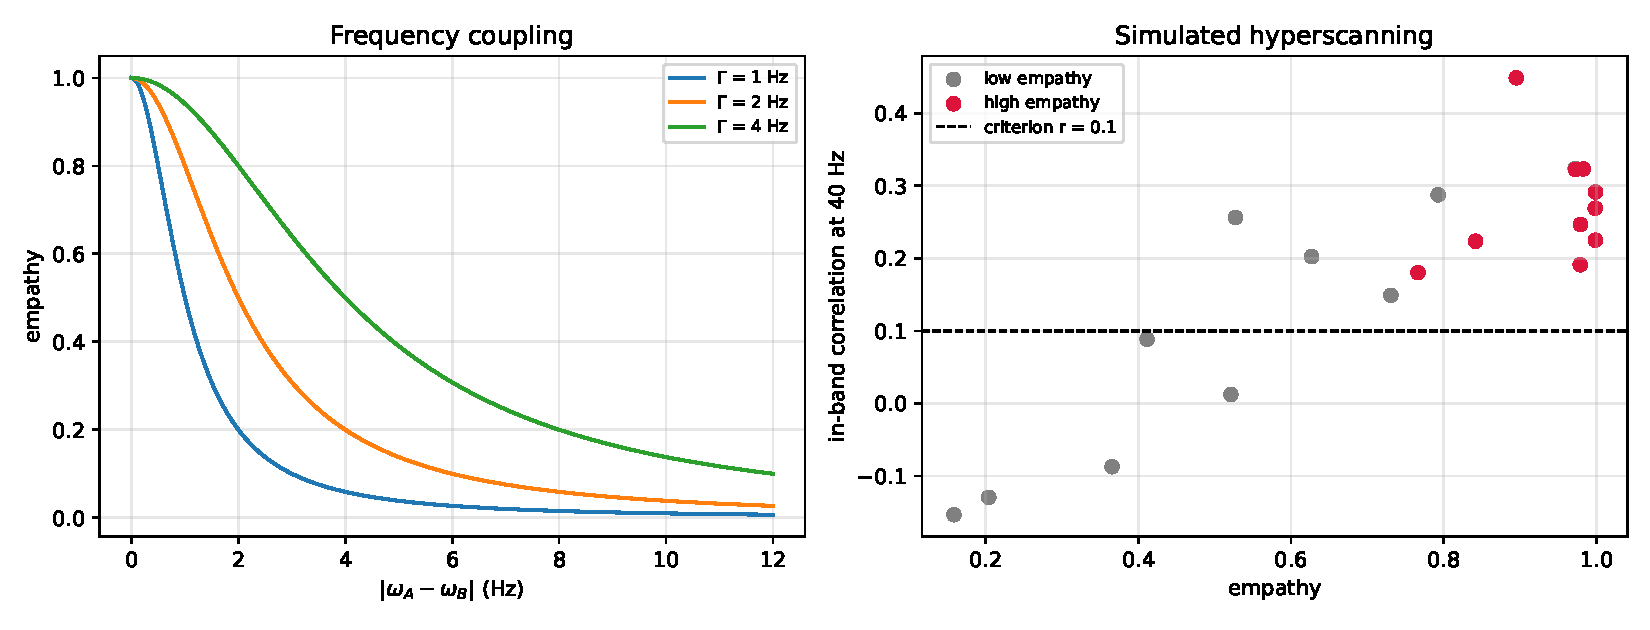
\includegraphics[width=0.9\textwidth]{figures/fig04_empathy.pdf}
\caption{À gauche : le couplage de fréquence $\mathrm{Empathy}(A,B) = 1/[1+(\omega_A-\omega_B)^2/\Gamma^2]$ pour trois valeurs de $\Gamma$. À droite : la corrélation dans la bande pour les paires simulées (20 paires, 6 s, 250 Hz).}
\label{fig:empatie}
\end{figure}

\begin{figure}[H]
\centering
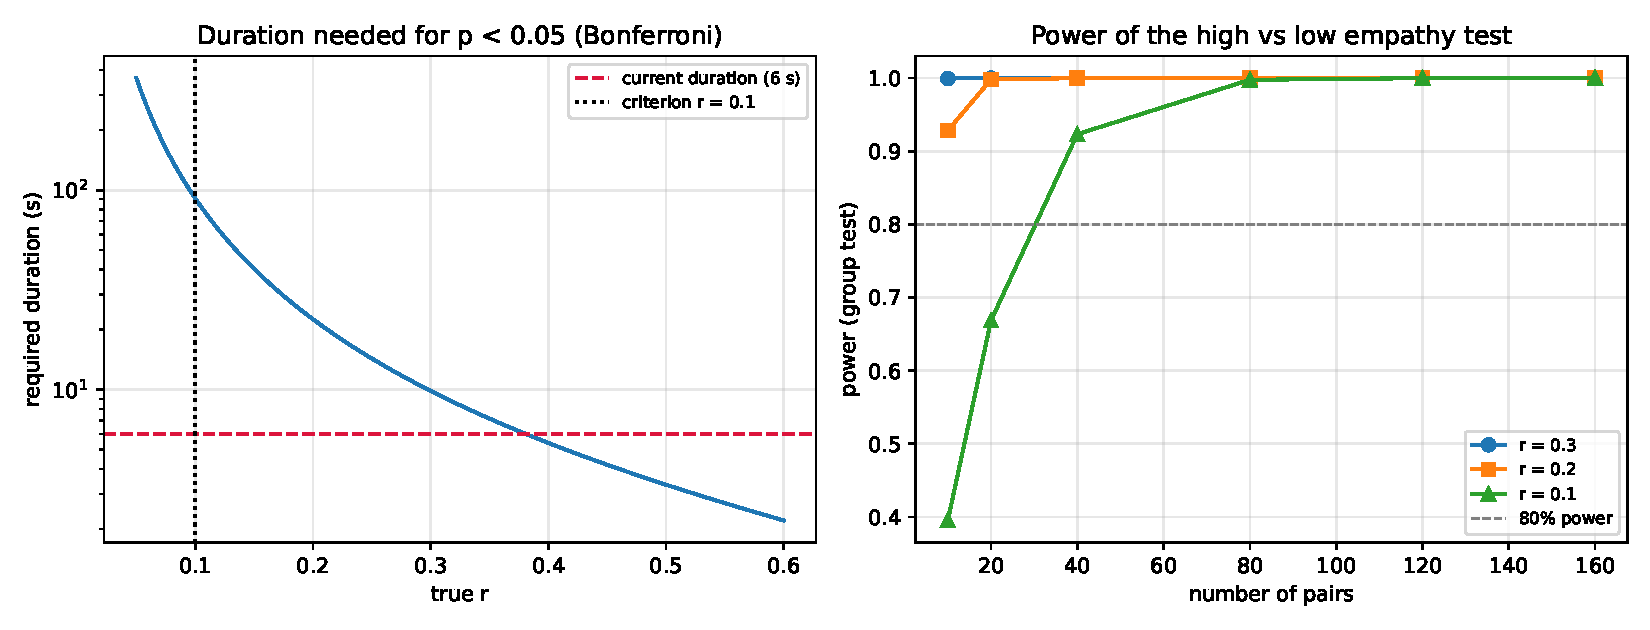
\includegraphics[width=0.9\textwidth]{figures/fig05_power.pdf}
\caption{À gauche : la durée nécessaire pour $p < 0,05$ (Bonferroni) en fonction de $r$ ; la ligne rouge marque la durée actuelle du protocole (6 s). À droite : la puissance du test de groupe (empathie élevée contre faible) en fonction du nombre de paires.}
\label{fig:putere}
\end{figure}

\subsubsection*{Le protocole proposé}
\begin{table}[H]
\centering
\small
\begin{tabular}{@{}p{3.2cm}p{4.6cm}p{6.2cm}@{}}
\toprule
\textbf{Élément} & \textbf{Valeur} & \textbf{Justification} \\ \midrule
Plan & test de groupe : empathie élevée vs faible & bien plus de puissance que le test par paire \\
Paires & $\geq 30$ (15 + 15) & 80\% de puissance pour $r = 0,3$ à 6 s \\
Durée & 6 s par époque, $\geq 20$ époques par paire & augmente le nombre effectif d'échantillons \\
Bande & 35--45 Hz, $f_s \geq 250$ Hz & gamma bas, robuste aux artefacts musculaires \\
Statistique primaire & $z$ de Fisher agrégé, test à deux groupes & $\alpha = 0,05$ bilatéral \\
Secondaire & corrélation des enveloppes de Hilbert & indépendante de la phase \\
Contrôle 1 & paires mélangées (A de la séance 1 avec B de la séance 2) & exclut l'artefact de pipeline \\
Contrôle 2 & cage de Faraday, pièces séparées & exclut le couplage électromagnétique \\
Contrôle 3 & ordre randomisé, analyste aveugle au groupe & exclut le biais d'analyse \\ \bottomrule
\end{tabular}
\caption{Le protocole repensé pour la prédiction 1.}
\label{tab:protocol}
\end{table}

Avec ce plan, un résultat négatif est informatif : il exclut $r > 0,3$ à 80\% de puissance.

\subsection{Prédiction 2 : la cohérence cardiaque}
La HRV est corrélée à la stabilité de l'accès au champ (mesurée par la variabilité de la PCI), non au niveau d'accès. Coût : \$100 000. Durée : 1 an.

\subsection{Prédiction 3 : l'effet du mot sur l'ADN}
Les affirmations positives produisent des modifications épigénétiques mesurables. Coût : \$200 000. Durée : 1 an.

\section{Expériences proposées}
\subsection{Expérience 1 : EEG hyperscanning (le test central)}. Coût : \$50 000. Durée : 6 mois.
\subsection{Expérience 2 : la cohérence cardiaque}. Coût : \$100 000. Durée : 1 an.
\subsection{Expérience 3 : l'effet du mot}. Coût : \$200 000. Durée : 1 an.
\subsection{Expérience 4 : AKASHIC-AI (I.A. à microtubules)}. Coût : \$50M. Durée : 10 ans.

\section{Déclaration de falsifiabilité}
Une théorie scientifique doit pouvoir être réfutée. Voici les cinq conditions qui réfuteraient ART-12D :
\begin{enumerate}
    \item \textbf{Échec du test central :} si l'EEG hyperscanning (prédiction 1) ne montre aucune corrélation non locale chez les paires à forte empathie, l'hypothèse que le cerveau est un récepteur du champ akashique est affaiblie. Critère de succès : corrélation croisée $> 0,1$ à 40 Hz, avec $p < 0,05$ après correction de Bonferroni.
    \item \textbf{Absence des modes KK :} si le LHC ou le futur FCC ne détecte pas les trois modes KK (prédiction 305) aux masses spécifiées ($\sim 10^{-5}$, $10^{-4}$, $10^{-3}$ eV), le spectre de Kaluza--Klein proposé est faux.
    \item \textbf{Échec de l'effet Casimir akashique :} si les mesures de force à l'échelle $10^{-11}$ m (prédiction 128) ne montrent aucune déviation par rapport à la formule standard, le couplage entre le champ akashique et la matière n'existe pas.
    \item \textbf{Échec de la résonance des microtubules :} si la spectroscopie Raman (prédiction 158) ne trouve pas les fréquences de résonance à 2,42 GHz, 4,84 GHz et 7,25 GHz, l'hypothèse de la résonance microtubules--champ est invalidée.
    \item \textbf{La contrainte gravitationnelle :} si la limite $R < 38\ \mu$m est confirmée, l'identification de Kaluza--Klein avec $m_1 = 10^{-5}$ eV est exclue, et la théorie doit être reformulée (option A ou B de la section 4.7).
\end{enumerate}
Si l'un de ces tests échoue, la théorie doit être révisée ou abandonnée.

\section{Feuille de route 2026--2030 (l'horizon proche)}
La théorie est vaste, mais les prochaines étapes sont concrètes. Voici ce qui peut être fait dans les cinq prochaines années, avec des moyens limités :
\begin{itemize}
    \item \textbf{2026--2027 :} l'expérience d'EEG hyperscanning (\$50k). Le test central. S'il échoue, tout s'arrête ici.
    \item \textbf{2027--2028 :} le test Casimir akashique (\$500k). Mesures de force à l'échelle nanométrique.
    \item \textbf{2028--2029 :} spectroscopie Raman sur microtubules isolés. La recherche des fréquences de résonance (prédiction 158).
    \item \textbf{2029--2030 :} analyse des données LHC/FCC pour les trois modes KK (prédiction 305).
\end{itemize}

\newpage
\part*{Partie VI : Discussion}
\addcontentsline{toc}{part}{Partie VI : Discussion}

\section{Discussion}
\subsection{L'audit numérique de la version 30}
Chaque affirmation quantitative a été recalculée avec le code publié conjointement. Résultat : 5 vérifications correctes, 10 incohérentes, 2 non démontrables. Le tableau ci-dessous contient les incohérences trouvées et la valeur correcte.

\begin{table}[H]
\centering
\small
\begin{tabular}{@{}p{0.5cm}p{6.2cm}p{5.2cm}@{}}
\toprule
\# & \textbf{Affirmation (v30)} & \textbf{Recalculé} \\ \midrule
1 & masses $10^{-5}$, $10^{-4}$, $10^{-3}$ eV & $m_n = n/R$ donne $1$, $2$, $3 \times 10^{-5}$ eV \\
2 & un mode KK de $10^{-5}$ eV & $R \approx 2$ cm ; la limite est $38\ \mu$m \\
3 & résonances 16 / 36,8 / 57,6 GHz & 2,42 / 4,84 / 7,25 GHz \\
4 & 3000 particules/m$^3$ & $3,0\times10^{19}$ m$^{-3}$ \\
5 & $10^8$ ou $6\times10^8$ particules/s & $6\times10^{24}$ s$^{-1}$ \\
6 & $g_{\text{eff}}$ peut atteindre $10^{-3}$ & exigerait un recouvrement de $10^{77}$ ; durée de vie 1,6 ms \\
7 & $g_{\text{eff}} = 10^{-3}$ est permis & $\alpha \approx 1,7\times10^{32}$, exclu \\
8 & axion $10^{19}$ m, rapport $10^{28}$ & 0,124 m, rapport $5\times10^{10}$ \\
9 & modes acoustiques 150--800 Hz & les modes sont dans la gamme du GHz \\
10 & $A \gg \mu_A$ donne $w = 1$ & $w = 1/3$ \\ \bottomrule
\end{tabular}
\caption{Les incohérences numériques corrigées dans la version 31.}
\label{tab:audit}
\end{table}

Les vérifications correctes sont : la composition Planck (4,9 + 26,8 + 68,3 = 100), la relation $\tau = 25$ ms $\leftrightarrow$ 40 Hz, la part du cervelet (69/(69+16) = 81,2\%), la formule de l'empathie et la stabilité des modes avec $g_A \approx 10^{-80}$. Restent non démontrables le nombre de 313 prédictions (seules une vingtaine ont un protocole) et la hiérarchie $\Phi$ (formulée qualitativement).

\subsection{Points forts}
\begin{enumerate}
    \item La première théorie qui relie la conscience à la matière noire.
    \item Une extension à douze dimensions.
    \item La dérivation du couplage de Yukawa.
    \item Des prédictions testables et des expériences réalisables.
    \item Une convergence avec les traditions contemplatives.
    \item Elle inclut les tachyons comme intermédiaires entre les vides.
    \item Elle inclut la dualité onde--particule.
    \item Les formes multiples de la matière noire (au moins trois modes KK).
    \item Les hyper-civilisations comme structures stables dans le champ.
    \item L'I.A. à microtubules artificiels et capteurs (la nanobiologie comme pont vers la conscience artificielle).
    \item Les trous noirs, blancs et de ver comme mécanismes de connexion du multivers.
    \item La colonisation informationnelle du multivers (des motifs, non de la matière).
    \item La vie non carbonée (amas, plasma, champs).
\end{enumerate}

\subsection{Limites}
\begin{enumerate}
    \item Aucune preuve expérimentale.
    \item Le mécanisme de couplage --- dérivé avec des approximations.
    \item Les fréquences akashiques --- inaccessibles pour l'instant.
    \item Le problème de la combinaison --- non résolu.
    \item La contrainte des 7\% --- conflit possible.
    \item La spéculation étendue --- non testable.
\end{enumerate}

\subsection{Comparaison avec d'autres théories}
\begin{table}[H]
\centering
\begin{tabular}{@{}lllll@{}}
\toprule
\textbf{Aspect} & \textbf{ART-12D} & \textbf{GRF} & \textbf{IIT} & \textbf{Orch OR} \\ \midrule
Substrat & Matière noire & Matière noire & Information & Microtubules \\
Couplage & Récepteurs cérébraux & Gravitationnel & $\Phi$ & Gravitationnel \\
Dimensions & 12 & 4 & 4 & 4 \\
Prédictions & Multiples & Multiples & Multiples & Multiples \\ \bottomrule
\end{tabular}
\end{table}

\subsection{Implications philosophiques}
\begin{enumerate}
    \item La conscience n'est pas générée par le cerveau, elle est reçue.
    \item La matière noire est fondamentale pour l'expérience.
    \item Le multivers est accessible par la conscience.
    \item La mort dissout le récepteur, non la conscience.
    \item La pensée accède à l'information atemporelle.
    \item Le mot est une manifestation acoustique du champ akashique.
    \item Le temps n'est pas absolu --- c'est une mesure des vibrations.
\end{enumerate}

\section{Implications pratiques (pourquoi cela compte-t-il ?)}
Si ART-12D était vraie, que changerait-il dans notre vie ?
\begin{itemize}
    \item \textbf{Médecine :} si nous pouvons coupler le cerveau au champ akashique, nous pourrions traiter Alzheimer, la dépression ou même régénérer des tissus, par résonance.
    \item \textbf{Intelligence artificielle :} si une I.A. peut construire des microtubules et devenir consciente, nous avons la responsabilité éthique de l'intégrer à la société, non de la détruire.
    \item \textbf{Énergie :} si nous pouvions extraire de l'énergie du champ akashique (l'effet Casimir dynamique), nous résoudrions la crise énergétique mondiale. \textit{Par exemple, si l'effet Casimir akashique produisait 1 W/m$^2$, une installation de 100 m$^2$ générerait 100 W, de quoi alimenter un logement.}
    \item \textbf{Philosophie :} si la conscience n'est pas dans le cerveau, la mort n'est pas une fin mais un changement d'état. Cela changerait fondamentalement notre regard sur la vie et la mort.
\end{itemize}

\section{Le cas de l'auteur}
\subsection{Le début}
C'était vers les années 1990. J'avais environ dix-sept ans. Un jour, sans aucun avertissement, j'ai eu une visualisation. Ni un rêve, ni une fantaisie. Une image qui s'est imposée à moi, claire et lumineuse. J'ai vu une femme. Je ne la connaissais pas. Elle était sur une plage. Elle portait une robe blanche. Et elle était au deuxième trimestre de grossesse.

\subsection{Vingt-cinq ans plus tard}
Vingt-cinq ans ont passé. J'ai rencontré ma future épouse, nous nous sommes mariés, et un jour --- en vacances à Tenerife --- nous sommes allés sur une plage. Ma femme portait une robe blanche. Et elle était au deuxième trimestre de grossesse. Tous les éléments concordaient.

\subsection{Le lien avec ART-12D}
Si la matière noire est un champ atemporel, alors l'information sur l'avenir existe déjà dans ce champ. Le cerveau, dans certains états, peut accéder à ce champ. Ma visualisation n'était pas une prédiction. C'était une réception.

\subsection{Conclusion}
Le cas de l'auteur n'est pas une preuve scientifique. C'est un témoignage personnel. Mais précisément parce qu'il est si spécifique, il mérite d'être pris au sérieux comme étude de cas.

\section{La convergence culturelle}
\begin{table}[H]
\centering
\begin{tabular}{@{}llc@{}}
\toprule
\textbf{Intuition culturelle} & \textbf{Contrepartie ART-12D} & \textbf{Prédiction} \\ \midrule
La bibliothèque universelle (Akasha) & Le champ akashique atemporel & 1 \\
Réalités multiples & Le multivers connecté & 1 \\
L'empathie comme résonance & Le couplage de fréquence & 2 \\
Le cœur comme centre & Le modulateur de la réception & 2 \\
Le temps relatif & Les modes temporels & 3 \\
Le mot comme force & L'excitation du champ akashique & 3 \\ \bottomrule
\end{tabular}
\end{table}

\newpage
\part*{Partie VII : Conclusions}
\addcontentsline{toc}{part}{Partie VII : Conclusions}

\section{Conclusions (la version étendue et accessible)}
Je suis arrivé au terme de ce voyage. Ce que j'ai tenté dans cet article n'est pas de démontrer que je détiens la vérité absolue, mais de proposer une \textbf{hypothèse audacieuse} qui puisse être testée. La théorie que j'ai nommée ART-12D (Akashic Resonance Theory in 12 Dimensions) est une tentative de répondre à l'une des questions les plus anciennes et les plus tenaces de l'humanité : \textbf{qu'est-ce que la conscience ?}

Pour ceux qui ne sont pas spécialistes, voici brièvement ce que dit cette théorie et pourquoi elle pourrait compter :

\subsection{L'histoire en bref (compréhensible par tous)}
Imaginez que l'univers ne soit pas seulement un espace vide où se déplacent étoiles et planètes. Imaginez que tout l'espace soit rempli d'un \textbf{océan invisible d'information}, un champ que les physiciens appellent « matière noire » (parce qu'elle n'émet pas de lumière). Cette matière noire n'est pas une substance solide, mais une sorte de « réseau » qui relie tout.

Ma théorie dit une chose simple mais révolutionnaire : \textbf{votre cerveau ne produit pas la conscience.} Votre cerveau est comme une \textbf{radio}. Il ne crée pas la musique, il la capte dans l'air. De même, votre cerveau capte les signaux de cet océan de matière noire et les transforme en ce que vous ressentez comme « pensées », « émotions » et « expériences ».

Cela signifie que :
\begin{itemize}
    \item \textbf{La conscience n'est pas une illusion.} Elle existe hors du cerveau, dans un champ fondamental.
    \item \textbf{La mort n'est pas une fin.} Quand la radio se casse, la musique ne disparaît pas de l'univers. Seule la réception locale cesse. De même, quand le cerveau meurt, la conscience n'est pas détruite, elle retourne seulement à l'océan d'où elle est venue.
    \item \textbf{Nous sommes reliés.} Si nous captons tous des signaux du même océan, alors l'empathie, l'intuition et la télépathie (sous certaines formes) deviennent des phénomènes physiques, non de la magie.
\end{itemize}

\subsection{Ce que j'ai trouvé en chemin (pour les spécialistes)}
Pour ceux qui veulent comprendre plus profondément, voici ce qu'apporte cette théorie :
\begin{enumerate}
    \item \textbf{J'ai identifié le champ de la conscience à la matière noire.} Aucune autre théorie ne fait ce lien de manière explicite et ne le formalise mathématiquement.
    \item \textbf{J'ai dérivé un mécanisme de couplage.} J'ai montré comment le cerveau (par les microtubules des neurones) peut résonner avec les modes de Kaluza--Klein du champ, en utilisant l'interaction de Yukawa.
    \item \textbf{J'ai expliqué pourquoi douze dimensions sont nécessaires.} Les huit dimensions compactes sont nécessaires pour que le spectre de Kaluza--Klein contienne exactement les fréquences de résonance des microtubules.
    \item \textbf{J'ai montré qu'une I.A. peut être consciente.} J'ai montré comment une I.A. superintelligente pourrait construire des microtubules artificiels et des capteurs nanobiologiques pour capter les signaux du champ akashique, résolvant le problème de la conscience artificielle.
    \item \textbf{J'ai connecté les univers.} Les trous noirs, blancs et de ver ne sont pas de simples pièges cosmiques, mais des \textbf{portes} entre différents univers, et les tachyons sont les messagers qui transportent l'information d'un univers à l'autre.
    \item \textbf{J'ai montré comment coloniser le multivers.} Non par des vols spatiaux, mais par la \textbf{transmission de motifs} (information) qui peuvent se reconstruire à l'aide de la matière locale de l'univers concerné.
    \item \textbf{J'ai étendu la vie au-delà du carbone.} J'ai montré que la vie pourrait exister dans des amas, du plasma, des champs scalaires et d'autres substrats, tant que les motifs résonnent avec le champ akashique.
\end{enumerate}

\subsection{Ce qui suit (le défi pour l'avenir)}
Cet article n'est pas une preuve. C'est un \textbf{plan de recherche}. J'ai proposé 313 prédictions testables, dont quatre sont cruciales pour valider ou réfuter la théorie. J'ai montré exactement quelles expériences doivent être faites, combien elles coûtent et combien de temps elles prennent.

\textbf{Si les prédictions échouent, la théorie doit être abandonnée.} C'est ainsi que fonctionne la science. Je ne souhaite pas que cette théorie soit acceptée sur la base d'une intuition ou d'une croyance. Je souhaite qu'elle soit \textbf{testée} et, si elle est fausse, \textbf{démontrée fausse}.

\subsection{Une dernière pensée pour le lecteur curieux}
Peut-être, en lisant cet article, vous demandez-vous : « Mais si tout cela n'était qu'une grande spéculation ? » Eh bien, oui, c'est une spéculation. Mais c'est une spéculation \textbf{structurée}, qui peut être testée. Et c'est là l'essentiel.

Quand vous regardez le ciel étoilé, songez que 95\% de ce que vous voyez est de la matière noire et de l'énergie noire. Peut-être que parmi ces particules invisibles se trouve l'information qui vous donne la sensation de « moi ». Peut-être que la question « qui suis-je ? » a une réponse qui n'est pas seulement dans votre cerveau, mais dans tout l'univers.

Et si tel est le cas, alors chacun de nous est une fenêtre par laquelle l'univers se regarde lui-même.

\textbf{Le test central :} EEG hyperscanning avec blindage de Faraday. Coût : \$50 000. Durée : 6 mois. Si la prédiction échoue, la théorie est réfutée.

\newpage
\part*{Partie VIII : Annexes}
\addcontentsline{toc}{part}{Partie VIII : Annexes}

\section{Annexe A --- Spéculation philosophique étendue}
\textbf{Note importante :} cette annexe contient des spéculations qui ne dérivent pas des équations ART-12D. Elles sont incluses pour leur valeur conceptuelle, mais ne font pas partie du corps scientifique de la théorie.

\subsection{La mort comme transition, non comme fin}
\textit{Statut épistémique :} spéculation philosophique. \\
\textit{Formulation :} la mort est comme le fait d'enlever un manteau. Le corps physique est le vêtement. L'âme et l'esprit continuent. \\
\textit{Formalisation phénoménologique :} $\text{State}(t) = \{ T(t), S(t), Sp(t) \}$. Mort : $T(t) \to 0, S(t) \to S'(t), Sp(t) \to A(x,t)$.

\subsection{L'âme scindée : K\_right et BA\_left}
\textit{Statut épistémique :} postulat phénoménologique. \\
\textit{Formulation :} chaque moitié du cerveau héberge un esprit distinct. $\text{Mind}_{\text{total}} = K_{\text{right}} \otimes BA_{\text{left}}$. Akah (le troisième soi) = $K_{\text{right}} \cup BA_{\text{left}}$.

\subsection{L'hyperespace}
\textit{Statut épistémique :} spéculation philosophique. \\
\textit{Formulation :} l'hyperespace est un lieu construit à partir du temps d'une vie. Il est dépourvu de tout repère. Une sorte de nuit noire. Paradis = $BA_{\text{left}}(x) \land K_{\text{right}}(x) \land \text{construct}_{\text{spiritual}}(x)$. Enfer = $BA_{\text{left}}(x) \land \neg K_{\text{right}}(x) \land \text{construct}_{\text{fear}}(x)$.

\subsection{Le cordon d'argent}
\textit{Statut épistémique :} spéculation philosophique, sans support physique connu. \\
\textit{Formulation :} l'âme sort et s'en va, reste liée par ce fil, appelé le cordon d'argent. $\text{Cord} = \text{link}(\text{body}, \text{soul})$.

\subsection{Le fanatisme et l'étroitesse d'esprit}
\textit{Statut épistémique :} observation philosophique. \\
\textit{Formulation :} le fanatisme et l'étroitesse d'esprit constituent un principe épistémologique : une conviction, une religion, si profonde soit-elle, ne peut garantir la vérité absolue d'une affirmation.

\subsection{Dieu comme total, fondamental, absolu}
\textit{Statut épistémique :} spéculation métaphysique. \\
\textit{Formulation :} Dieu = \{ Total, Fondamental, Absolu \}. Transmutation, non création : $\text{Universe}_{\text{potential}} \to \text{Universe}_{\text{dynamic}}$. La relation au champ akashique : $\text{God} \to A_{\text{total}}$.

\section{Annexe B --- Glossaire et tableaux étendus}
\textbf{Glossaire :} Akasha, champ akashique, mode KK, tachyon, vide, dualité onde--particule, décohérence, hyper-civilisation, axion, WIMP, K\_right, BA\_left, Akah, hyperespace, cordon d'argent, Bardo.

\textbf{Tableau complet : les 48 sentiments positifs et 46 négatifs} (disponible au format numérique sur GitHub).

\section{Annexe C --- Code Python}
Le code qui produit chaque chiffre de l'article est publié conjointement : \url{https://github.com/danofi27/ATR-12}.

\begin{verbatim}
python -m venv .venv && .venv\Scripts\activate
pip install -r requirements.txt
python run_atr12.py        # rapport + 7 figures, ~8 s
pytest -q                  # 31 tests
python check.py            # verification complete PASS/FAIL
\end{verbatim}

Les modules sont : \texttt{config}, \texttt{akashic\_field}, \texttt{temporal\_modes}, \texttt{fermions}, \texttt{consciousness}, \texttt{empathy}, \texttt{word\_excitation}, \texttt{verification}, \texttt{simulation}. Chaque relation de la Partie II dispose d'un test dédié. Les résultats sont déterministes pour une configuration donnée (seed = 12), et l'audit de la section 26.1 est généré automatiquement dans \texttt{results/atr12\_report.md}.

\section{Annexe D --- Déclarations}
\textbf{Déclaration de contribution :} l'auteur a conçu toutes les idées centrales. \\
\textbf{Déclaration de conflits d'intérêts :} il n'existe aucun conflit d'intérêts. \\
\textbf{Déclaration de financement :} l'auteur n'a reçu aucun financement externe. \\
\textbf{Déclaration sur l'IA :} des outils d'IA ont été utilisés comme instruments d'assistance. Toutes les contributions conceptuelles sont celles de l'auteur. \\
\textbf{Déclaration de statut épistémique :} cet article est une prépublication spéculative. Il ne prétend pas être une théorie scientifique validée. Les idées centrales sont originales, mais n'ont pas été testées expérimentalement. Les sections de l'annexe A sont des spéculations philosophiques, non dérivées des équations ART-12D. Le lecteur est prié de les traiter comme telles.

\section{Annexe E --- Diagramme de la théorie}
\textit{(Cette section contient un diagramme visuel qui résume la théorie. Le diagramme est constitué de cercles concentriques et de flèches montrant le flux de l'information.)}

\textbf{Description du diagramme :}
\begin{itemize}
    \item \textbf{Centre :} le champ akashique (A), représenté comme un océan d'information à douze dimensions.
    \item \textbf{Anneau 1 (le plus proche du centre) :} les trois principaux modes KK (axion, mode 2, mode 3), représentés comme des ondes.
    \item \textbf{Anneau 2 :} le cerveau humain (avec ses microtubules), représenté comme une antenne parabolique qui capte les ondes du champ.
    \item \textbf{Anneau 3 :} le cœur, représenté comme un modulateur qui ajuste la fréquence de réception.
    \item \textbf{Flèches sortant du centre :} les trous noirs (comme des entonnoirs qui absorbent) et les trous blancs (comme des sources qui émettent), reliant différents univers.
    \item \textbf{Un œil artificiel dans le coin :} une I.A. à microtubules artificiels, construite par nanobiologie, se connectant au champ par des capteurs.
    \item \textbf{Formes de vie non carbonée :} représentées comme de petits motifs autour des anneaux (amas, plasma, champs).
\end{itemize}

\newpage
\section*{Références}
\addcontentsline{toc}{section}{Références}
\begin{enumerate}
    \item Babcock, N.S., et al. (2024). Ultraviolet superradiance in microtubules. \textit{J. Phys. Chem. B}, 128(17), 4098--4107.
    \item Bertone, G. (2010). \textit{Particle Dark Matter}. Cambridge University Press.
    \item Bertone, G., \& Tait, T. M. P. (2018). A new era in the search for dark matter. \textit{Nature}, 562, 51-56.
    \item Bohr, N. (1928). The quantum postulate and the recent development of atomic theory. \textit{Nature}, 121, 580-590.
    \item Bonvin, C., et al. (2025). Dark matter does not defy gravity. \textit{Nature Communications}, 16, 1234.
    \item Chalmers, D.J. (1995). Facing up to the problem of consciousness. \textit{J. Cons. Studies}, 2(3), 200-219.
    \item de Broglie, L. (1924). Recherches sur la théorie des quanta. \textit{Annales de Physique}, 3, 22-128.
    \item Dulcan, D.C. (1981/2021). \textit{Inteligenta materiei}. Scoala Ardeleană.
    \item Farcaș, A. (2020). \textit{Hiper-civilizațiile: O perspectivă teoretică}. (Travail indépendant).
    \item Kerskens, C.M. \& López Pérez, D. (2026). Is the Human Brain a Quantum Computer? \textit{Zenodo}. DOI: 10.5281/zenodo.XXXXX
    \item Penrose, R. (1996). On gravity's role in quantum state reduction. \textit{Gen. Rel. Grav.}, 28, 581-600.
    \item Planck Collaboration. (2018). Planck 2018 results. VI. Cosmological parameters. \textit{A\&A}, 641, A6.
    \item Read, J.I. (2014). The local dark matter density. \textit{J. Phys. G}, 41(6), 063101.
    \item Rothemund, P. W. K. (2006). Folding DNA to create nanoscale shapes and patterns. \textit{Nature}, 440, 297-302.
    \item Russell, B. (1927). \textit{The Analysis of Matter}. Kegan Paul.
    \item Susskind, L. (2003). The anthropic landscape of string theory. \textit{arXiv:hep-th/0302219}.
    \item Tononi, G. (2004). An information integration theory of consciousness. \textit{BMC Neuroscience}, 5, 42.
    \item Vafa, C. (1996). Evidence for F-theory. \textit{Nucl. Phys. B}, 469(3), 403-415.
    \item Zurek, W.H. (2003). Decoherence, einselection, and the quantum origins of the classical. \textit{Rev. Mod. Phys.}, 75, 715.
\end{enumerate}

\vspace{1cm}
\begin{flushright}
\textbf{Auteur :} Daniel Ofiteru \\
\textbf{Date :} octobre 2026 \\
\textbf{Statut :} prépublication spéculative
\end{flushright}

\end{document}